%!TEX TS-program = xelatex
%!TEX encoding = UTF-8 Unicode
\documentclass[headsepline, bibtotoc]{scrbook}

% \usepackage{fancyhdr}
% \usepackage{caption}[2008/08/24] % fuer captions in Figures
% \usepackage{scrpage2} % fuer Kopf- und Fusszeilenlayout
% \usepackage{titlesec} % um das Layout von Ueberschriften zu aendern

% \documentclass[a4paper, twoside, headsepline, 11pt, BCOR10mm, DIV10, footinclude, headinclude]{scrbook}
% \documentclass[a4paper, twoside, headsepline, 11pt, BCOR10mm, DIV10, footinclude, headinclude]{scrbook}
% BCOR: ``binding correction'' am besten an einem Probedruck ausmessen
% DIV:  beinflusst, wie ``gross'' der Satzspiegel wird -- s. Koma-Dokumentation
% footinclude, headinclude: dadurch werden die Fuss- und Kopfzeilen
%       in den Satzspiegel eingebunden (empfiehlt sich bei lebendenden

\synctex=1
\usepackage{marvosym}
\usepackage{upgreek}
\usepackage{gensymb}
\usepackage{stmaryrd}
\usepackage{amssymb} % Mathe
\usepackage{amsmath} % Mathe
\usepackage[usenames,dvipsnames]{color}
\usepackage{algorithmic}
\usepackage{algorithm}
\floatname{algorithm}{Algorithmus}
\renewcommand{\listalgorithmname}{Algorithmenverzeichnis}
\usepackage{listings}
\lstdefinelanguage{Javascript} {
morekeywords     = {
break,const,continue,delete,do,while,export,for,in,function,
if,else,import,in,instanceOf,label,let,new,return,switch,this,
throw,try,catch,typeof,var,void,with,yield
},
sensitive        = false,
morecomment      = [l]{//},
morecomment      = [s]{/*}{*/},
morestring       = [b]",
morestring       = [d]'
}
\lstset{
language         = Javascript,
frame            = tb,
framesep         = 5pt,
basicstyle       = \footnotesize\ttfamily,
showstringspaces = false,
keywordstyle     = \ttfamily\bfseries\color{CadetBlue},
identifierstyle  = \ttfamily,
stringstyle      = \ttfamily\color{OliveGreen},
commentstyle     = \color{MidnightBlue},
rulecolor        = \color{Gray},
xleftmargin      = 5pt,
xrightmargin     = 5pt,
aboveskip        = \bigskipamount,
belowskip        = \bigskipamount
}

% Math Fonts
%\usepackage[mathcal]{eulervm}
\usepackage{eulervm}
\usepackage[cm-default]{fontspec}
% FONTS
\usepackage{xunicode}
\usepackage{xltxtra}
\defaultfontfeatures{Mapping=tex-text} % converts LaTeX specials (``quotes'' --- dashes etc.) to unicode
\setromanfont [Ligatures={Common}, Numbers={OldStyle}]{Adobe Caslon Pro}
\setmonofont[Scale=0.8]{Monaco}
% \setsansfont[Scale=0.9]{Optima Regular}
\setsansfont[Scale=0.9]{Myriad Pro}
% ---- CUSTOM AMPERSAND
\newcommand{\amper}{{\fontspec[Scale=.95]{Adobe Caslon Pro}\selectfont\itshape\&}}

\newcommand{\TODO}{\textsc{\textbf{\textcolor{red}{Todo\ }}}}
\newcommand{\FIXME}{\textsc{\textbf{\textcolor{red}{Fixme\ }}}}

% HEADINGS
% \usepackage{sectsty}
% \usepackage[normalem]{ulem}
% \sectionfont{\sffamily\mdseries\large}
% \subsectionfont{\rmfamily\mdseries\scshape\normalsize}
% \subsubsectionfont{\rmfamily\bfseries\upshape\normalsize}

% PDF SETUP
% ---- FILL IN HERE THE DOC TITLE AND AUTHOR
\usepackage[
xetex,bookmarks,colorlinks,breaklinks,
pdftitle={Detexify: Erkennung handgemalter LaTeX-Symbole},
pdfsubject={LaTeX-Symbolerkennung},
pdfauthor={Daniel Kirsch}
]{hyperref}
\hypersetup{linkcolor=blue,citecolor=blue,filecolor=black,urlcolor=blue}

% Stuff
\usepackage[ngerman]{babel}
\usepackage{indentfirst}
\usepackage[printonlyused]{acronym}
\usepackage{url}
\usepackage[numbers,square]{natbib}
\usepackage{wrapfig}

% \pagestyle{headings}
%

\hyphenation{Mannig-faltig-keit}

\begin{document}

\titlehead{{\Large Westfälische Wilhelms-Universität Münster \hfill Institut für Informatik}}
\title{Detexify: Erkennung handgemalter \LaTeX-Symbole \\
\vspace{5mm} 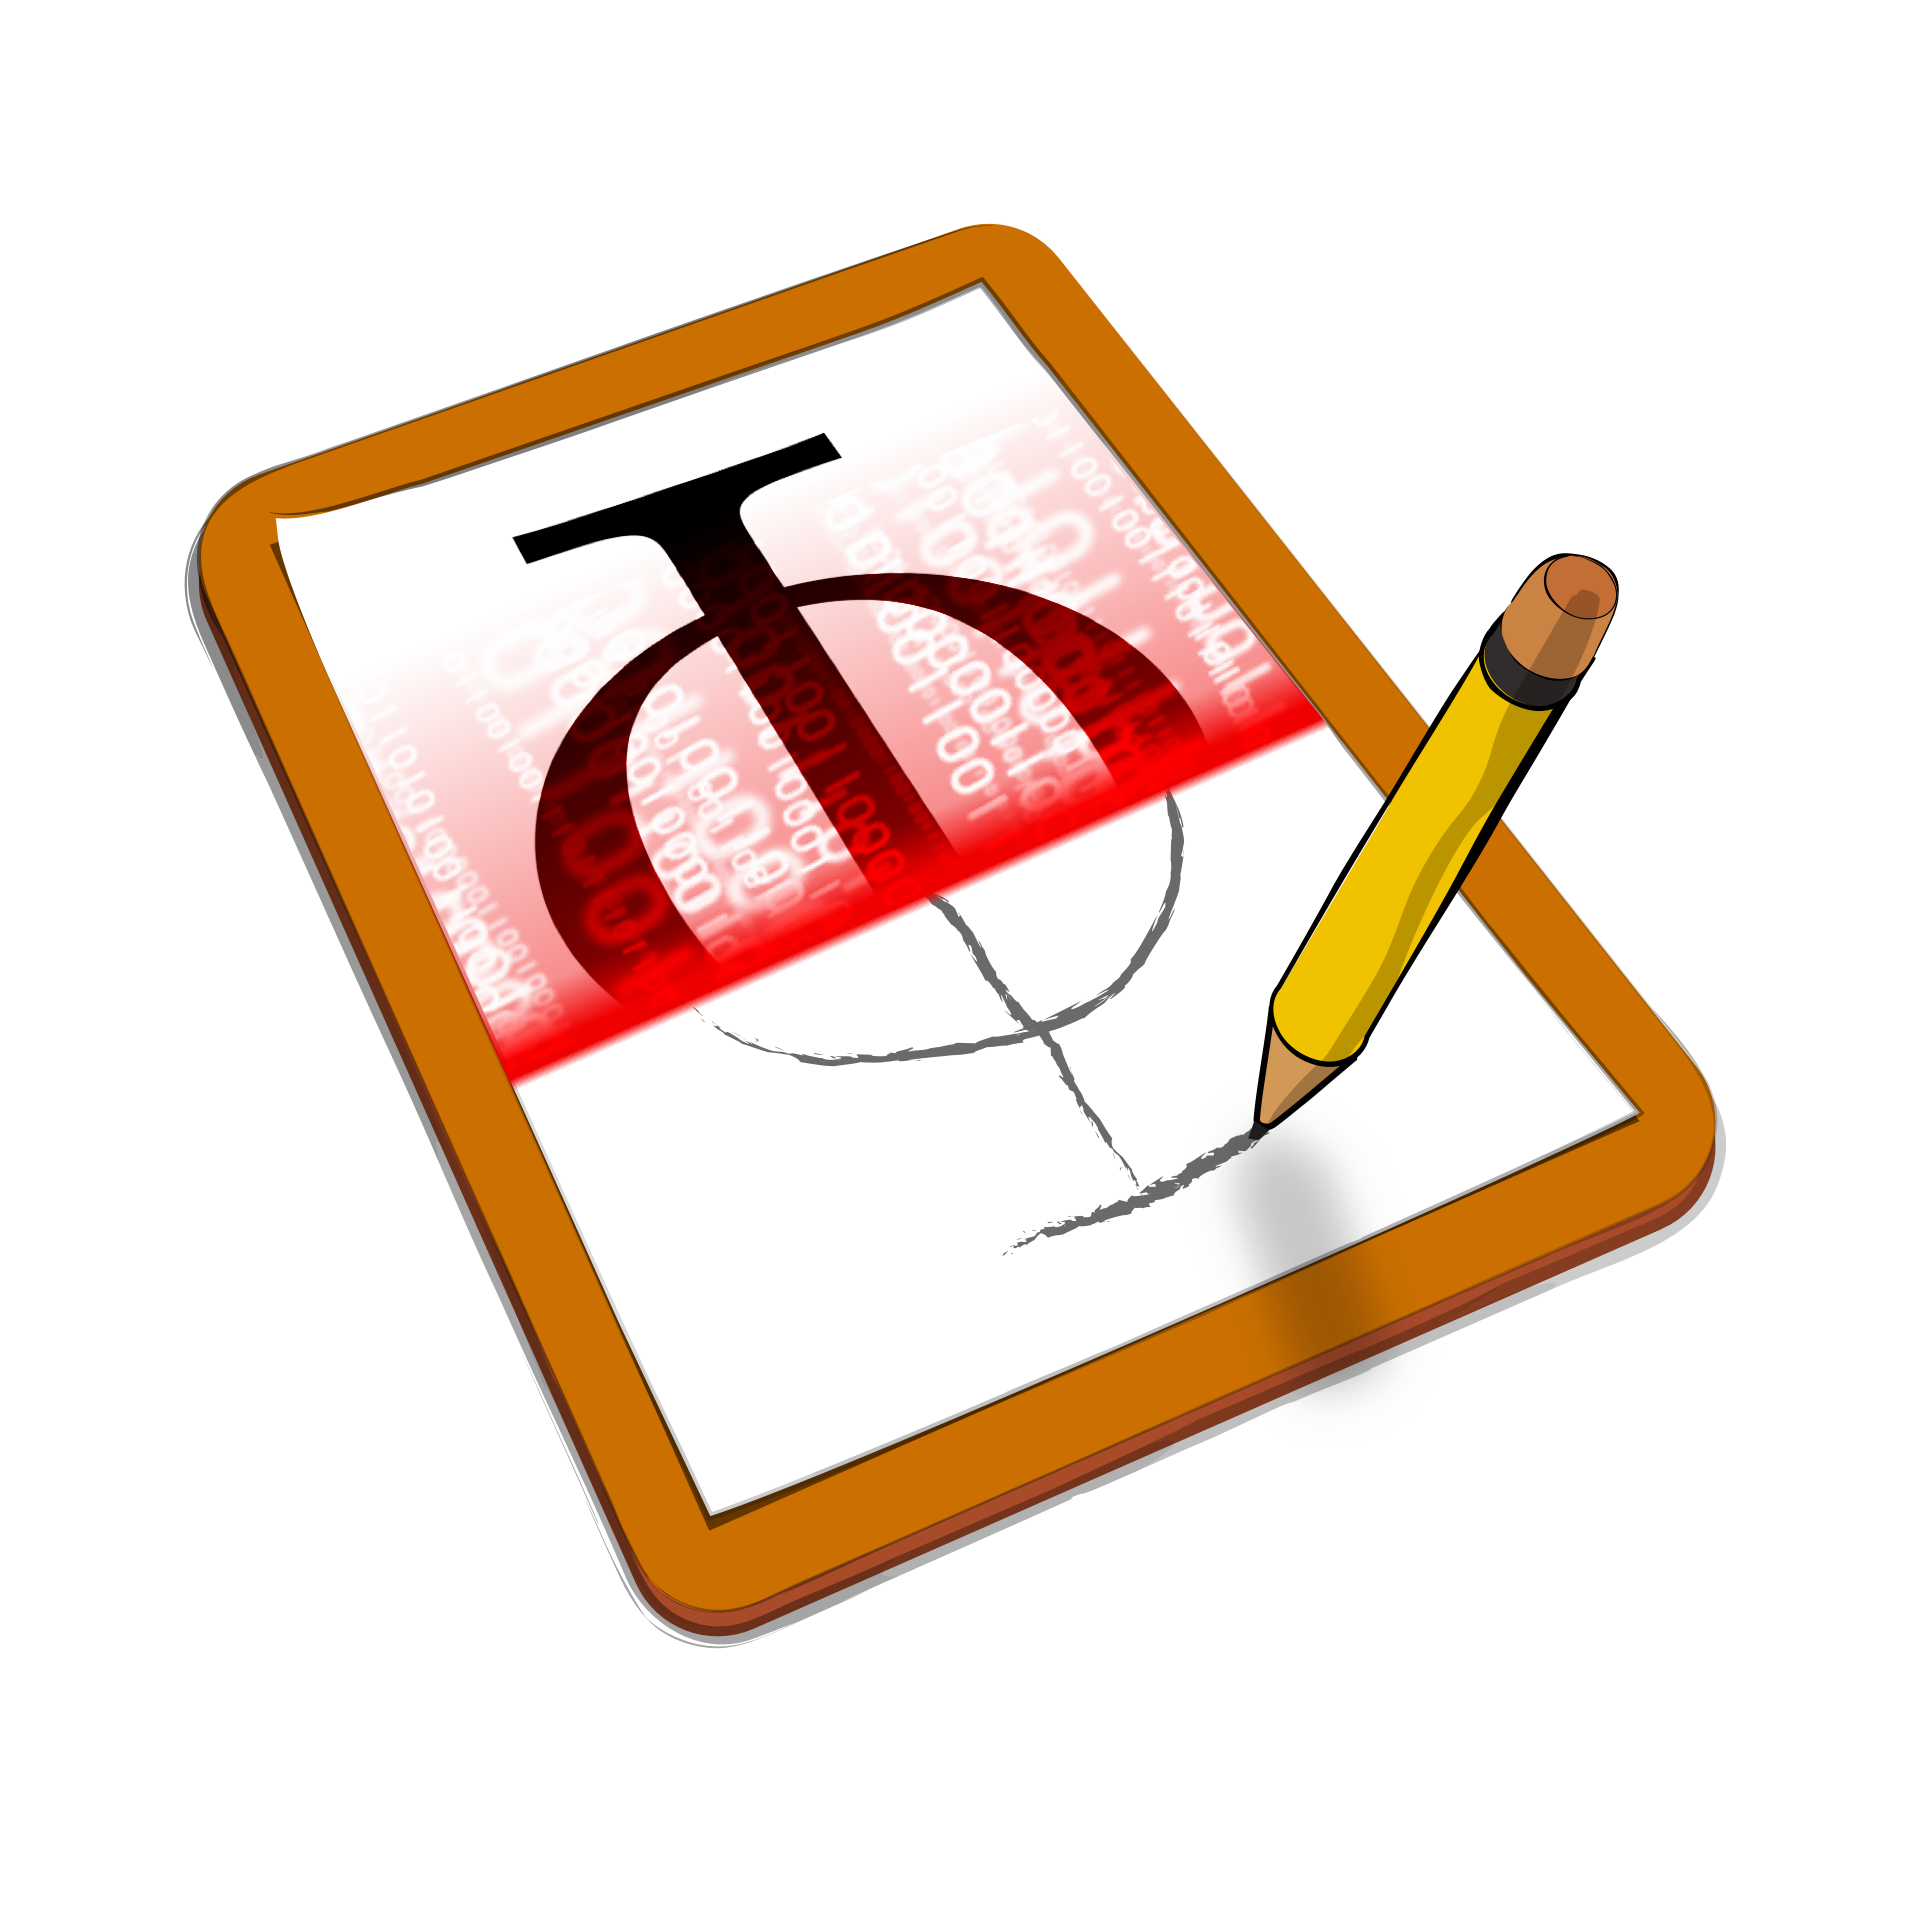
\includegraphics[height=7.5cm]{figures/icon.png} }

\subject{Diplomarbeit}
\author{Daniel Kirsch}
\date{\today}
\publishers{Betreut durch Prof. Dr. Xiaoyi Jiang}

\maketitle

\frontmatter

% \newpage\mbox{}\vfill
% \begin{center}
% \large
% 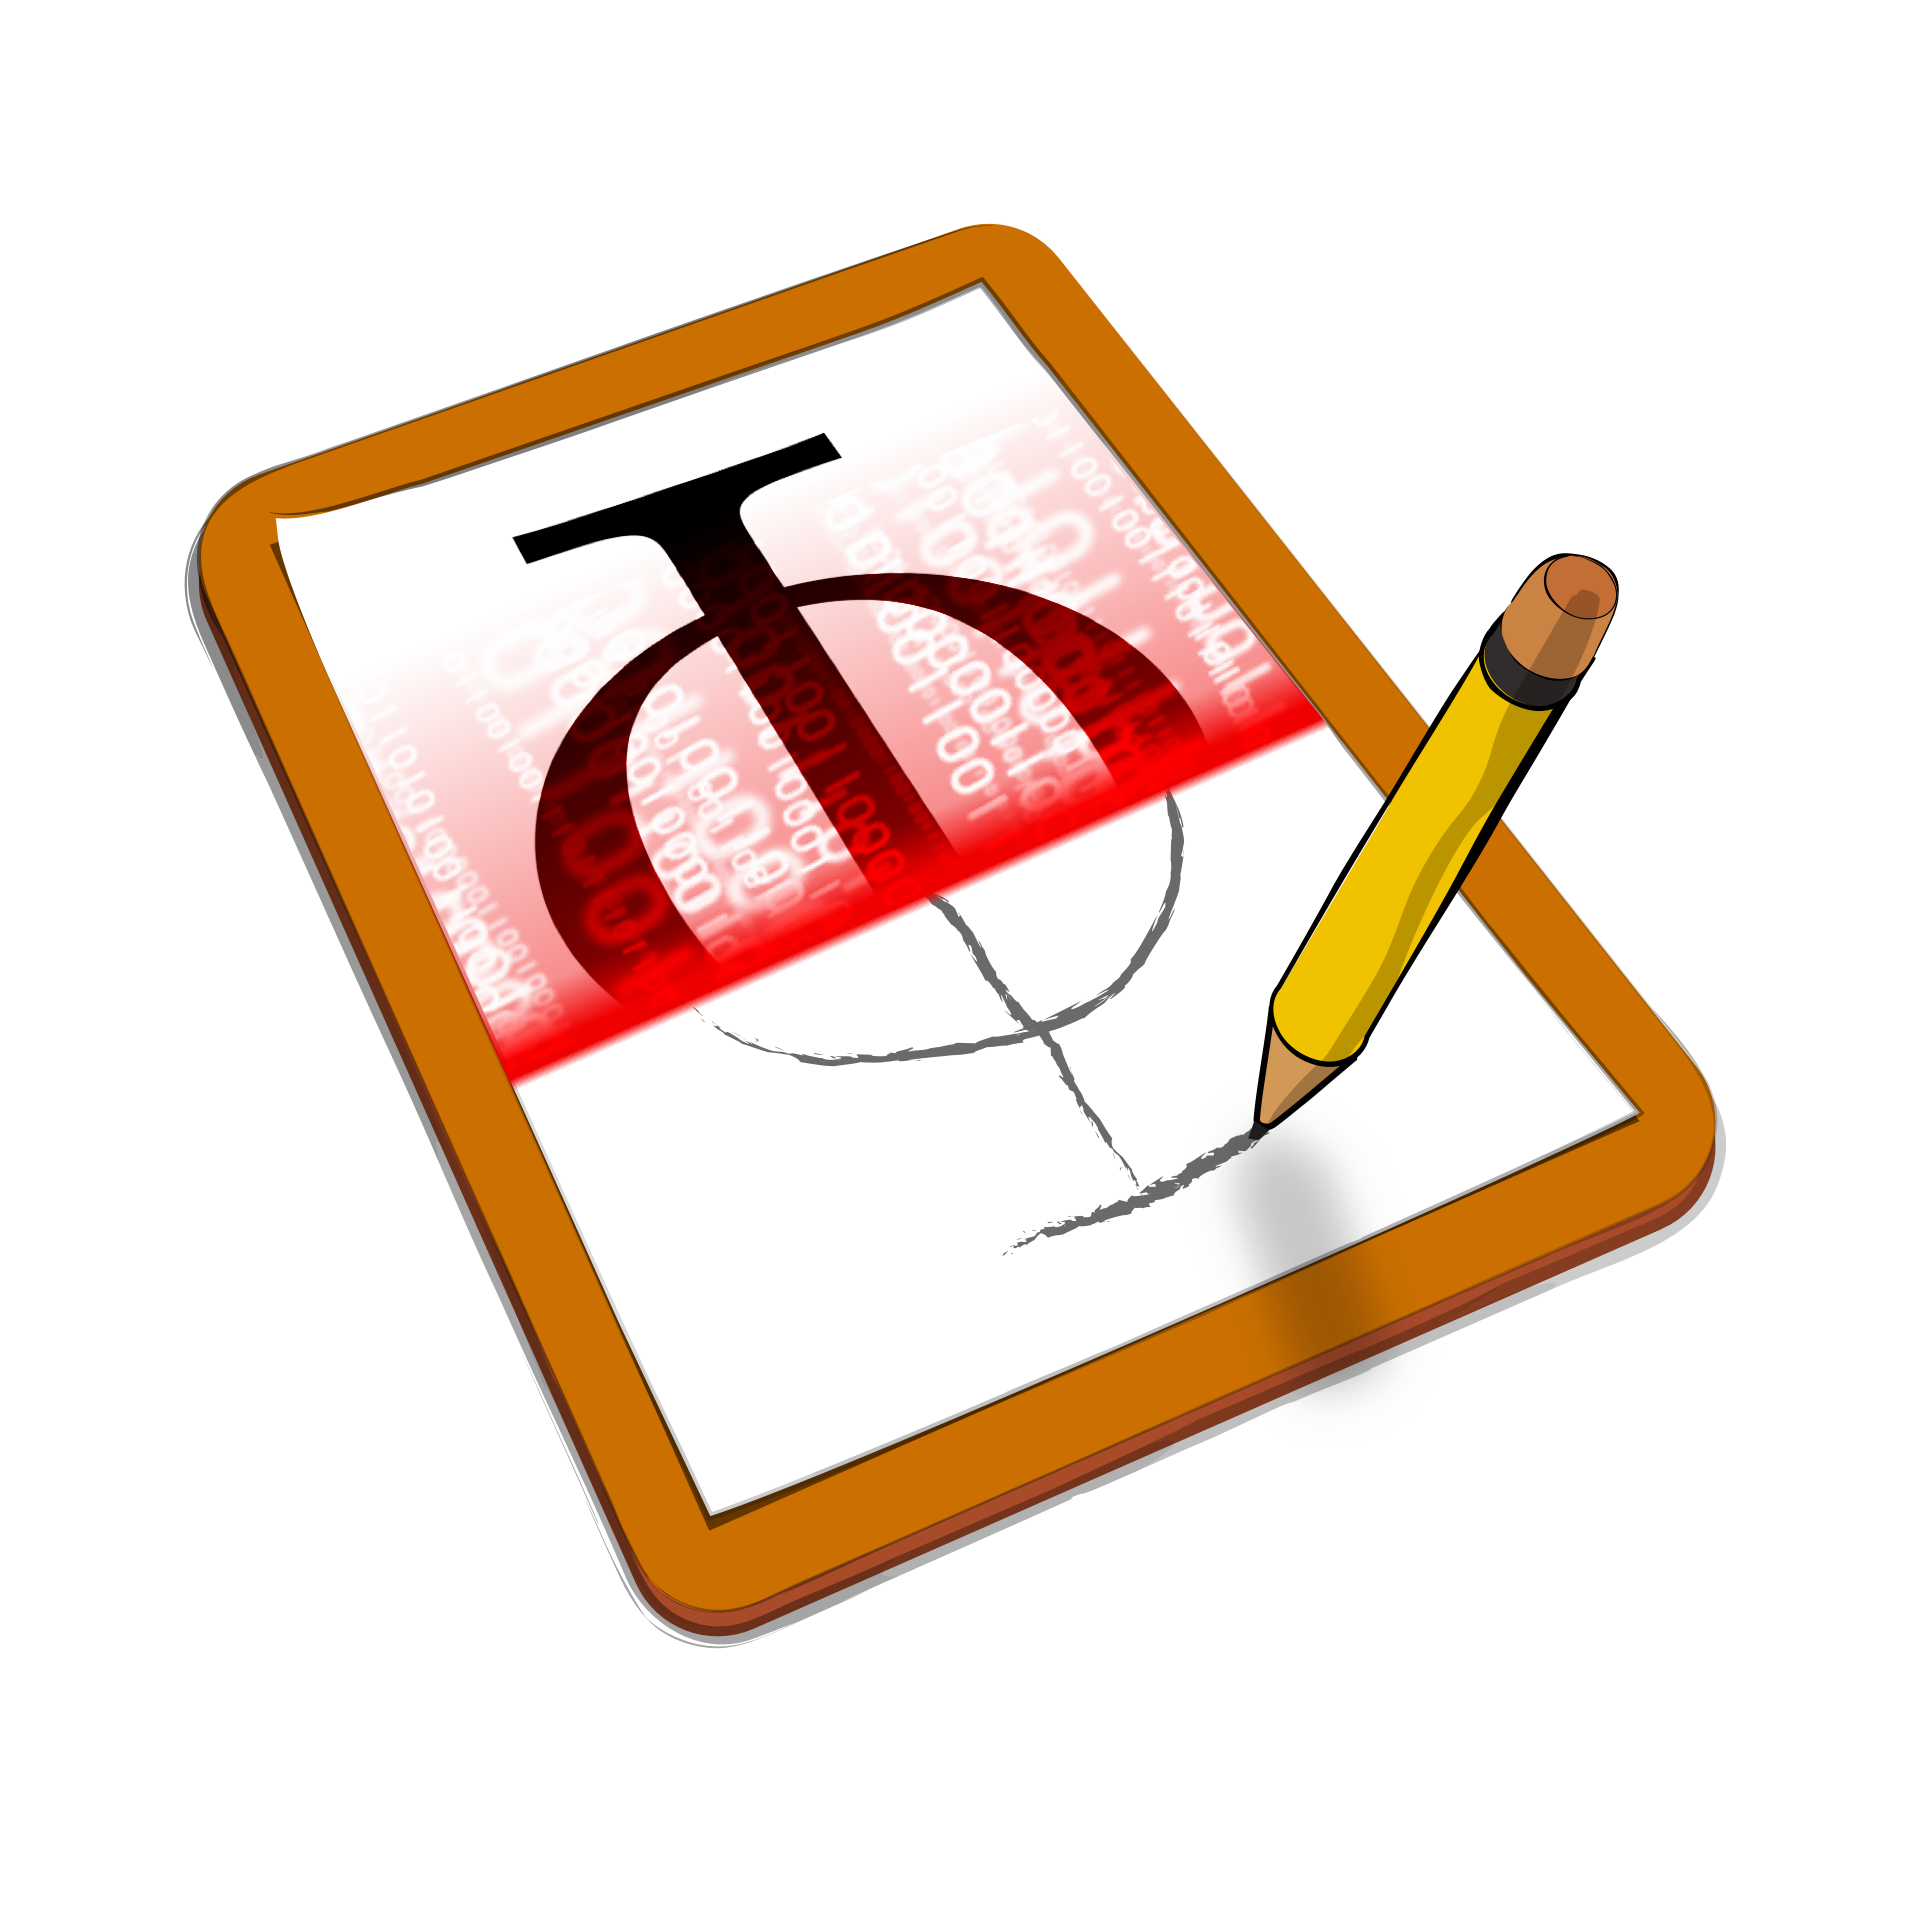
\includegraphics{figures/icon.png}
% \normalsize
% \end{center}
% \vfill\mbox{}\newpage

%\rule{0mm}{1mm}
%\newpage
\pagestyle{empty}
\cleardoublepage
\chapter{Statement of authorship}

\setlength{\parindent}{0mm}
I hereby certify that this diploma thesis has been composed by myself, and describes my own work, unless otherwise acknowledged in the text. All references and verbatim extracts have been quoted, and all sources of information have been specifically acknowledged. It has not been accepted in any previous application for a degree.\\

\vspace{20mm}

Münster, \today\\

\vspace{15mm}

Daniel Kirsch\\
% \rule{0mm}{1mm}
% \newpage
\pagestyle{empty}
\cleardoublepage


% Fürs Prüfungsamt ein paar Seiten frei.
\pagestyle{headings}

\tableofcontents  % Inhaltsverzeichnis

\chapter{Vorwort}

\section*{Wie es zu dieser Diplomarbeit kam}

Eines Tages saß ich mit einem Kommilitonen zusammen in der Mensa. Wir unterhielten uns über Ideen im Allgemeinen und welche es sich lohne umzusetzen. Wir hatten viele Ideen und meistens keine Zeit sie zu verwirklichen. Tatsächlich existierte sogar eine Liste mit einigen davon - ein schlichtes Blatt Papier, auf dem sich über die Zeit einiges angesammelt hatte und wir nannten es den Ideenfriedhof.

Am besagten Tag ging es vor allem darum, wie man auf {\em gute} Ideen käme. Denn auf dem Ideenfriedhof ruhte Sinnvolles und weniger Sinnvolles. Ich äußerte die Behauptung, dass Ideen, die eigene Probleme lösen, solche seinen, deren Umsetzung sich lohne, weil man in der Regel mit seinen Problemen nicht alleine dastehe. Somit löse man auch Probleme für andere.

Wir kamen auf andere Themen und da mein Kommilitone zu jener Zeit den Sketretärinnen seiner Arbeitsgruppe einen \LaTeX-Kurs gab, unterhielten wir uns auch darüber. Irgendwann bemerkte er: "`Da fällt mir etwas ein... Was fehlt ist eine LaTeX-Rückwärts-Suche. Es kommt ganz häufig vor, dass man zwar weiss, was man für ein Symbol haben will, aber nicht den Befehl kennt. Das Problem hatten meine Sekretärinnen jetzt auch schon ein paar Mal. Wenn man jetzt ein Programm hätte, in das man das Symbol malen könnte und das dann den richtigen Befehl ausspuckt..."'

Ich fand, dass das einen außergewöhnlich gute Idee war. Ich hatte das Problem zwar nicht selbst, aber ich würde es bald haben, wenn ich meine Diplomarbeit schreiben würde, denn ich würde sie in \LaTeX\ schreiben. Ich hatte allerdings zu dem Zeitpunkt noch keine Ahnung, was ich als Diplomarbeit schreiben würde. Ich hatte zu diesem Zeitpunkt auch keine Berührung mit Mustererkennung irgendeiner Art gehabt und keine Ahnung von \LaTeX. Ich fand aber das Problem so interessant, dass ich fest entschlossen war es anzugehen.

Einige Wochen später, nach vielem Lesen und Probieren, hatte ich eine benutzbare Version, implementiert als Webseite und bedienbar über einen Webbrowser. Seitdem wird die Anwendung täglich von fast 800 Besuchern genutzt. Erst als diese Arbeit getan war, ist mir klar geworden, dass sich das Thema doch ganz gut für eine Diplomarbeit eignet und zu meiner Freude war Prof. Jiang auch dieser Meinung. Zudem würde ich meine eigene Diplomarbeit bei der Erstellung meiner Diplomarbeit verwenden können. Wer kann das schon von sich behaupten?

Was aber ich eigentlich hier sagen will: Sie lesen nun im wesentlichen das Ergebnis eines \LaTeX-Kurses für Sekretärinnen der Arbeitsgruppe Topologie des Mathematischen Institutes der WWU Münster. Darum gilt den damaligen TeilnehmerInnen mein besonderer Dank.
\mainmatter
%!TEX root = /Users/daniel/Documents/thesis/thesis.tex
\chapter{Motivation}

\section{\LaTeX}

Wenn es um das Verfassen wissenschaftlicher Texte geht, ist für viele \LaTeX\ die erste Wahl. Anders als bei einem \acs{WYSIWYG}-Editor kümmert man sich nicht um das Layout, um Abstände und Schriftgrößen sondern um die Semantik des Geschriebenen. Stattdessen zeichnet man die Kapitel, Abschnitte, Formeln usw. semantisch aus, eher wie in \acs{HTML}. Der Vorteil liegt klar auf der Hand. Inhalt und Präsentation sind klar getrennt, was zur Folge hat, dass man nicht vom Wesentlichen abgelenkt wird, wenn man an Texten und Formeln arbeitet, und dass das Aussehen des Dokuments zentral in der Präambel definiert wird.

\LaTeX\ hat jedoch auch seine Nachteile. Gerade Anfänger haben es aufgrund der flachen Lernkurve schwer. Da man \LaTeX\ in der Regel im Quelltext bearbeitet, als jeden Befehl von Hand schreibt. Muss man sich unheimlich viel merken. Das beginnt bei einfachen Befehlen wie \texttt{\textbackslash chapter}, deren Name sich geradezu aufdrängt, aber wenn es darum geht Mathematische Formeln wie $$\Gamma \left( x \right) = \int\limits_0^\infty  {s^{x - 1} e^{ - s} ds}$$ in das Dokument zu bringen, wird es schon schwieriger.

Dass man ein $\Gamma$ mit dem Befehl \texttt{\textbackslash Gamma} bekommt ist noch zu erahnen. Um $\infty$ zu bekommen hätte man auch \texttt{\textbackslash infinity} statt \texttt{\textbackslash infty} versuchen können und hätte bloß eine Fehler geerntet, aber bei Befehlen wie \texttt{\textbackslash leftrightsquigarrow} ($\leftrightsquigarrow$) hört jede Intuition auf. Es ist also offensichtlich, dass es einigen Raum für unterstützende Maßnahmen bei der Erstellung von \LaTeX-Dokumenten gibt. Das gilt insbesondere für mathematische Formeln in denen viele unterschiedliche Symbole vorkommen können.

\section{Die optimale Eingabemethode}

Überlegt man sich die natürlichste Art Text oder Mathematik zu notieren, so kommt man unweigerlich auf Stift und Papier. Während bei Texten die Eingabe über eine Computertastatur durchaus schneller sein kann, als das Schreiben mit einem Stift (TODO Belege!) ist spätestens bei Formeln klar, dass hier der Stift klar im Vorteil ist. Es können beliebige Formen, Zeichen und Symbole in beliebige räumliche Beziehung gebracht werden. Nichts liegt also näher, als diese Eingabeform in die digitale Welt übertragen zu wollen.

Als Eingabegerät bietet sich also ein Grafiktablett an. Ein entsprechender \LaTeX-Editor würde eine Fläche zur Verfügung stellen, auf die einfach geschrieben und skizziert wird. Die Kurven und Linien würden dann vom Editor in Text, Tabellen, Formeln und Diagramme überführt -- alles genau wie vom Benutzer erwartet. Leider sind wir noch nicht so weit.

Alleine der Bereich der mathematischen Formelerkennung ist noch nicht auf einem Level, auf dem man die verfügbaren Lösungen als benutzbar bezeichnen könnte. Ein Beispiel ist die kostenlose Software \href{http://www.inftyproject.org}{InftyEditor}. Einfache Formeln werden noch recht sicher erkannt, aber sobald die Komplexität der Formel steigt und vor allem sobald man Symbole braucht, die die Software gar nicht kennt, wird die Benutzung zum Frusterlebnis. Es wundert daher nicht, dass an diesem Problem viel aktuelle Forschung betrieben wird.

\TODO{Beispiele oder Zitate/Referenzen}

Das Problem teilt sich dabei in drei Teile auf. Das erste ist die Segmentierung der mathematischen Formel, bei der einzelne Symbole isoliert werden müssen. Als zweites müssen die einzelnen Symbole richtig erkannt werden. Schließlich müssen die Symbole über ihre räumliche Position in eine logische Beziehung zueinander gebracht werden. Diese in diesen Schritten gewonnenen Erkenntnisse können natürlich die Entscheidung in den jeweils anderen beeinflussen, indem man die Semantik einer Interpretation in der Erkennung mit einfließen lässt. \TODO Zitate? Das Problem ist also sehr komplex.

\TODO{Hier könnte ein wenig Forschungsübersicht gegeben werden}

\section{Suche nach Alternativen}

Die optimale Eingabemethode ist also (noch) nicht praktikabel. Um ganze Formeln zu erkennen haben wir noch nicht die optimalen Algorithmen gefunden. Eine Alternative ist, dem Computer nur einen Teil der Erkennung zu übertragen. Ein Beispiel hierfür ist \href{http://jequation.sourceforge.net/}{JEquation}. In diesem Programm wird dem Benutzer vorgegeben, wo der zu malen hat, damit die Struktur der Formel richtig erkannt wird. \TODO Bild? Es bleibt also die Aufgabe die einzelnen Symbole zu erkennen.



\href{http://lyx.org}{Lyx}


\section{Ein pragmatischer Ansatz}



\url{http://url.de}
%!TEX root = /Users/daniel/Documents/thesis/thesis.tex
\chapter[Detexify]{Detexify - \LaTeX-Symbolsuche als Webanwendung} % (fold)
\label{cha:detexify}

Bevor ich auf die technischen Details von Detexify eingehe sollten Sie, lieber Leser, sich kurz mit dem Programm vertraut gemacht haben. Die Beschreibungen sind dann viel verständlicher. Die Benutzung von Detexify sollte selbsterklärend sein. Sollten Sie doch Schwierigkeiten haben finden Sie in \ref{man:benutzerhandbuch} ein kurzes Benutzerhandbuch. Sie können auf Detexify mit einem modernen Browser\footnote{Aktuelle Versionen von Firefox, Chrome, Safari und Opera \TODO IE testen.} unter der Adresse \url{http://detexify.kirelabs.org} zugreifen.

Die folgenden Abschnitte enthalten neben der Beschreibung der Funktionalität von Detexify außerdem Hinweise zur Implementierung.

\section{Architektur} % (fold)
\label{sec:architektur}

Bei jeder Anwendung muss man sich, bevor sie geschrieben wird, entscheiden, wie die Anwendung zur Verfügung gestellt werden soll. Daraus resultieren weitere Entscheidungen, wie z.B. die Wahl der Programmiersprache und der Datenformate.

Detexify wurde als Webanwendung implementiert. Dies hat die folgenden Vorteile:

\begin{itemize}
  \item \textbf{Plattformunabhängigkeit:} Heutzutage ist ein Webbrowser auf jedem Computer verfügbar. Um Detexify verwenden zu können wird nur ein moderner\footnotemark[1] Webbrowser benötigt.
  \item \textbf{Zentrale Wartung:} Fehlerbehebungen und Verbesserungen sind zentral anwendbar und stehen jedem Benutzer beim nächsten Besuch der Anwendung sofort zur Verfügung.
  \item \textbf{Zentrale Trainingsdaten:} Die Trainingsdaten sind zentral in einer Datenbank gespeichert. Das Training der Klassifizierers wird von den Nutzern selbst durchgeführt (siehe auch \ref{sec:crowdsourcing}).
\end{itemize}

Dabei besteht Detexify aus zwei lose gekoppelten Komponenten und zwar der Webanwendung und der Klassifizierungsserver (Server). Lose Kopplung heisst dabei, dass lediglich ein Interface definiert ist, wie die Webanwendung mit dem Server zu kommunizieren hat. (\TODO loose coupling in der Literatur) Das Interface ist als \ac{REST}-Interface spezifiziert. Die beiden Komponenten kommunizieren also über \ac{HTTP}. Abbildung~\ref{fig:architecture} zeigt die Architektur schematisch.

\begin{figure}
  \centering 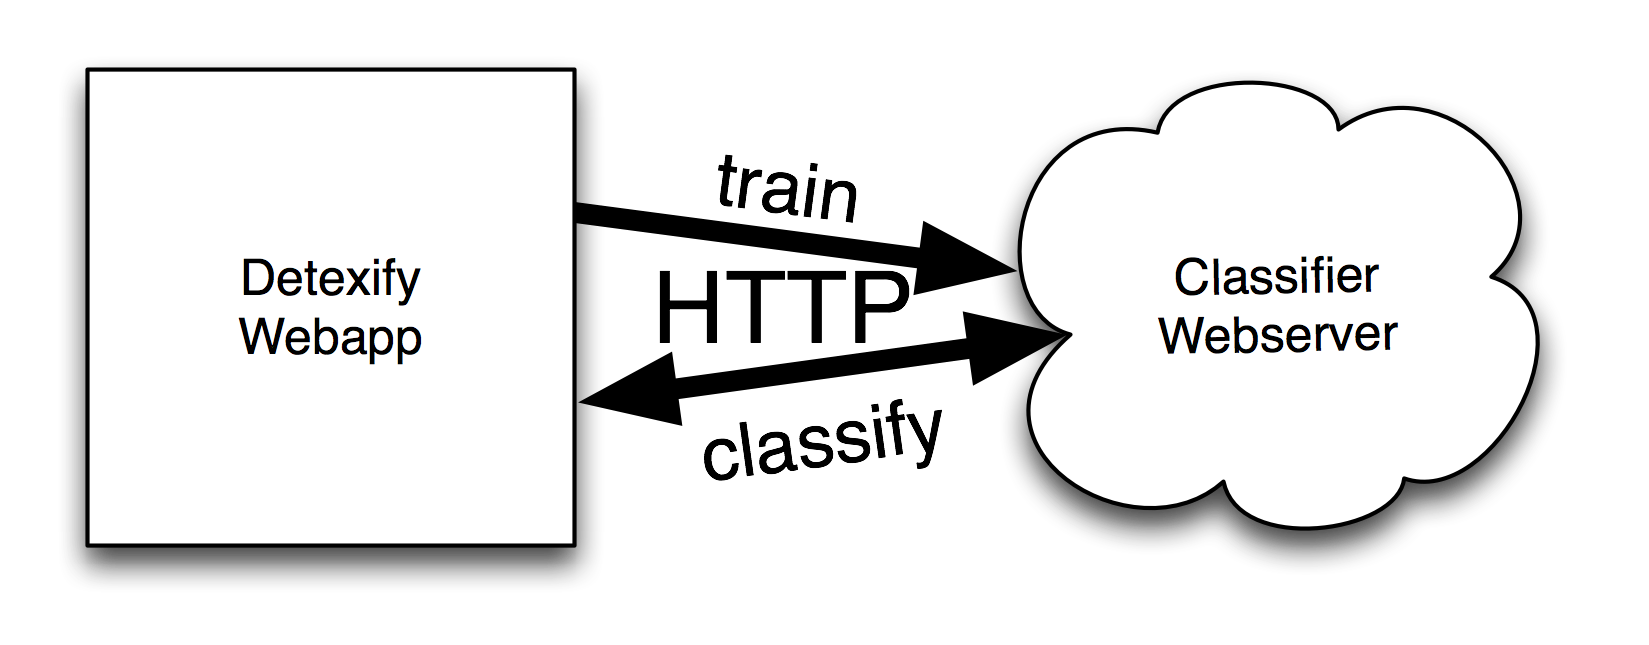
\includegraphics{figures/architecture.pdf}
  \caption{Detexify Architektur}
  \label{fig:architecture}
\end{figure}

\section{Server} % (fold)
\label{sec:server}

Der Server übernimmt die Mustererkennung. An ihn können im wesentlichen zwei verschiedene Anfragen gestellt werden. Die erste davon ist das Training einer Symbolklasse. Die zweite ist die Klassifizierung von unbekannten Daten. Es gibt noch eine dritte Anfrage, die aber lediglich zur Identifizierung und Statusermittlung der Serverimplementierung dient.

Da der Server die eigentliche Arbeit verrichtet läuft er auf einem leistungsstarken Rechner. \TODO Wieso keine Parallelisierung, wo wir doch eh schon in der Wolke sind...

Das \ac{REST}-Interface\footnote{Genauere Erklärungen zu \ac{REST} findet der Leser in \ref{sec:rest}} sieht folgendermaßen aus:

\subsection{REST-Interface} % (fold)
\label{sub:rest_interface}

\subsubsection{Training}

Um eine Symbolklasse zu trainieren müssen dem Server der Bezeichner der Klasse und die Trainingsdaten übergeben werden. Der Bezeichner ist dabei Teil der \ac{URL} und die Trainingsdaten werden als \ac{JSON}\footnote{Siehe \ref{sec:json}}-String im \ac{HTTP}-Request-Body übertragen.

\begin{lstlisting}[caption={Anfrage}]
  POST /train/{id}
  application/json
  [[{"x":12.3, "y":4.56, "t":7890},...],...]
\end{lstlisting}
\begin{lstlisting}[caption={Antwort}]
  200 OK
\end{lstlisting}
\begin{lstlisting}[caption={Antwort im Fehlerfall}]
  422 Unprocessable Entity
  application/json
  { "error" : "error message" }
\end{lstlisting}

\subsubsection{Erkennung}

Zur Erkennung werden die unbekannten Daten als \ac{JSON}-String an den Server übertragen. Dies geschieht wie beim Training im \ac{HTTP}-Request-Body. Als Antwort erhält die Webanwendung eine \ac{JSON}-kodierte Liste von Klassenbezeichnern und einer zugehörigen Wertung. Je kleiner die Wertung, desto wahrscheinlicher die zugehörige Klasse.

\begin{lstlisting}[caption={Anfrage}]
  POST /classify
  application/json
  [[{"x":12.3, "y":4.56, "t":7890},...],...]
\end{lstlisting}
\begin{lstlisting}[caption={Antwort}]
  200 OK
  application/json
  [{ "id" : "key", "score": 1.234}, ...]
\end{lstlisting}
\begin{lstlisting}[caption={Antwort im Fehlerfall}]
  422 Unprocessable Entity
  application/json
  { "error" : "error message" }
\end{lstlisting}

\subsubsection{Serverstatus}

Durch die lose Kopplung durch das hier definierte Interface lässt sich der Server leicht austauschen\footnote{Tatsächlich existieren Serverimplementierungen in drei verschiedenen Programmiersprachen.} und um die verwendete Serverimplementierung identifizieren zu können gibt es noch eine dritte Anfrage, die aber zur Funktionalität des Servers nichts beiträgt.

\begin{lstlisting}[caption={Anfrage}]
GET /
\end{lstlisting}
\begin{lstlisting}[caption={Antwort}]
200 OK
application/json
{ 
  "server" : "server string to identify implementation",
  "version" : "version string e.g. 1.0"
}
\end{lstlisting}
  
% subsection rest_interface (end)

% section server (end)

\section{Webanwendung} % (fold)
\label{sec:webanwendung}

% section webapp (end)

Die Webanwendung stellt das Benutzerinterface von Detexify dar. Sie wird über einen Browser bedient. Es gibt zwei Sichten (jeweils durch statische \ac{HTML}-Seiten realisiert.) Die erste Sicht ermöglicht die Symbolsuche und die zweite Sicht bietet eine Symboltabelle aller in Detexify registrierten \LaTeX-Symbole. In dieser können die Symbole auch trainiert werden.

\subsection{Symbolsuche} % (fold)
\label{sub:symbolsuche}

Die Symbolsuche ist das Zentrum der Anwendung. Sie ist das Werkzeug, das dem \LaTeX-Entwickler das Leben vereinfachen soll. Abbildung~\ref{fig:symbolsuche} zeigt einen Screenshot eines Browsers mit geöffneter Symbolsuche.

Auf der Seite der Webanwendung ist dafür eine Zeichenfläche implementiert. Auf dieser können mit der Maus Striche gemalt werden, und nach jedem beendeten Strich wird per AJAX\footnote{Siehe \ref{sec:ajax}} eine Erkennungsanfrage an den Server gesendet. Die Symbole werden dann anhand der vom Server ermittelten Rangfolge aufgelistet wie in Abbildung~\ref{fig:symbolsuche} zu sehen. Die Kommunikation erfolgt wie in \ref{sec:server} erwähnt über das Datenformat \ac{JSON}. Die Interaktion ist mithilfe von Javascript gelöst. Die Zeichenfläche basiert auf der \ac{SVG}-Technologie.

\begin{figure}
  \centering 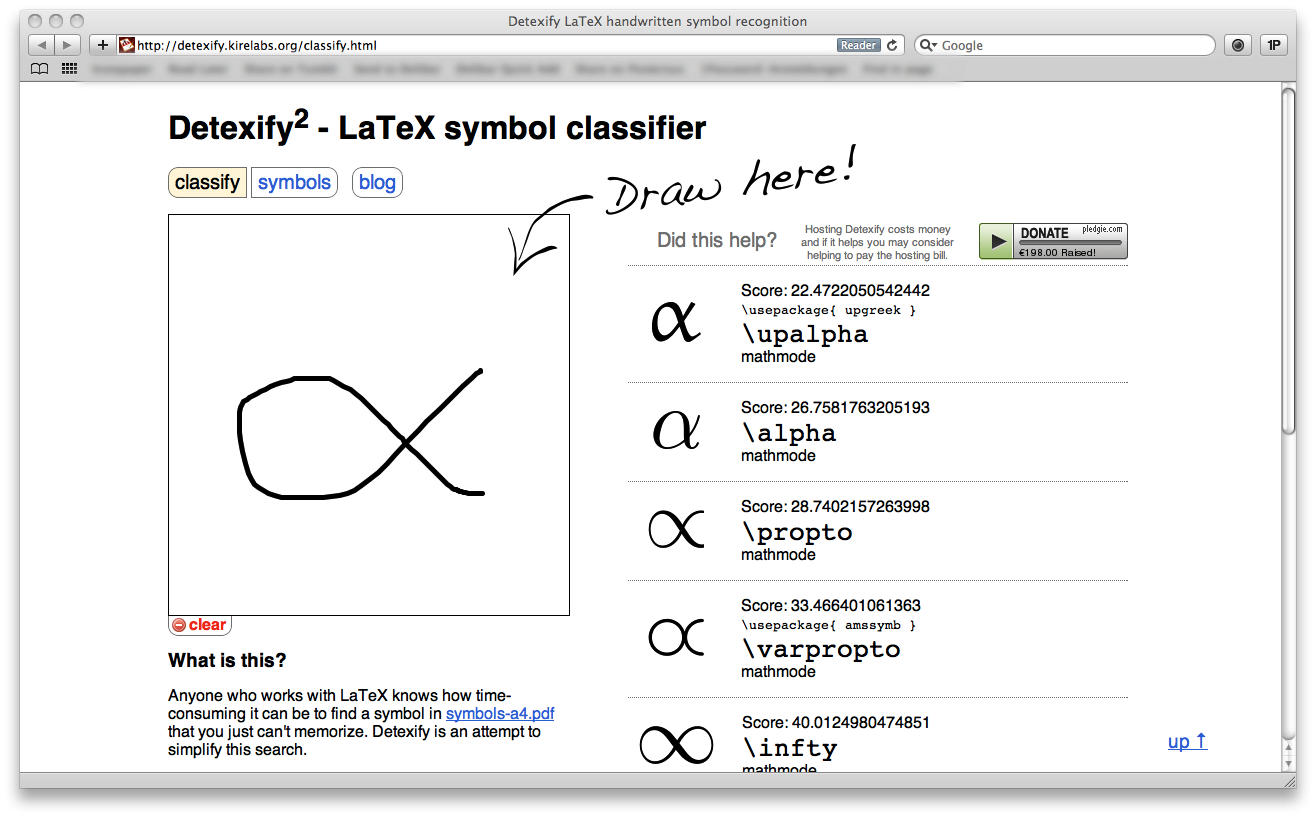
\includegraphics[width=\textwidth]{figures/interface-classify.png}
  \caption{Symbolsuche}
  \label{fig:symbolsuche}
\end{figure}

% subsection symbolsuche (end)

\subsection{Symboltabelle} % (fold)
\label{sub:symboltabelle}

Einerseits bietet die Symboltabelle einen Überblick über die in Detexify registrierten und damit über die Symbolsuche auffindbaren Symbole. Andererseits bietet die Symboltabelle durch ihre Sortierungs- und Filtermöglichkeiten von sich aus gute Möglichkeiten zur Symbolsuche, sollte die eigentliche Symbolsuche aus irgendwelchen Gründen versagen. Außerdem können in der Symboltabelle geziehlt einzelne Symbole trainiert werden. Die Funktionalität der Symboltabelle ist im Detail in \ref{man:symboltabelle} beschrieben. Die verwendeten Technologien sind sind identisch mit den bei der Symbolsuche verwendeten.
 Abbildung~\ref{fig:symboltabelle} zeigt einen Screenshot eines Browsers mit geöffneter Symboltabelle.

\begin{figure}
  \centering 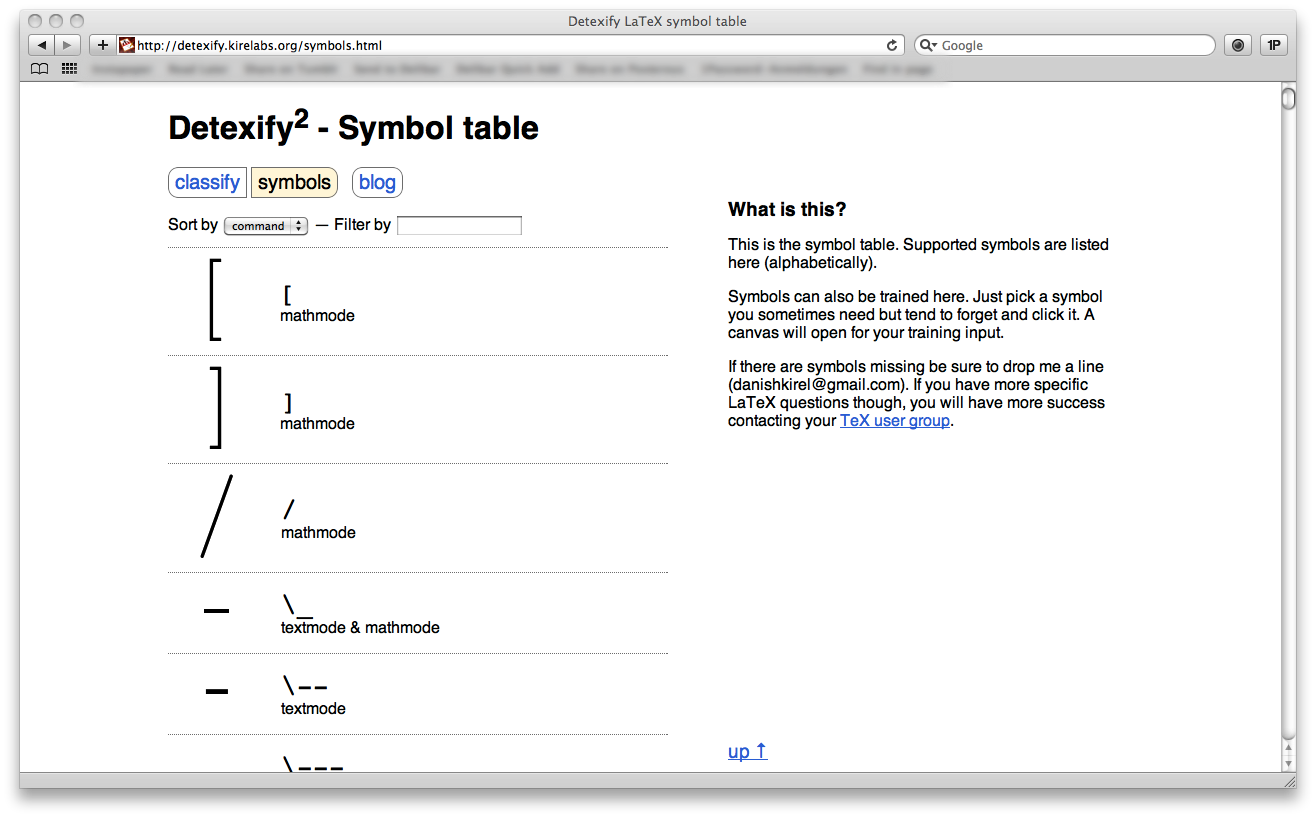
\includegraphics[width=\textwidth]{figures/interface-symbol-table.png}
  \caption{Symboltabelle}
  \label{fig:symboltabelle}
\end{figure}

% subsection symboltabelle (end)


\section{Crowdsourcing des Trainings} % (fold)
\label{sec:crowdsourcing}

Wie in \ref{sub:symboltabelle} erwähnt bietet Detexify den Nutzern ein Interface um das Training durchzuführen. Tatsächlich habe ich nie ein initiales Training vorgenommen. Der Plan war von Anfang an, das Training vollständig den Nutzern zu überlassen. So eine Vorgehensweise nennt man Schwarmauslagerung (Crowdsourcing) \TODO Literatur. Die Überlegung war dabei die Folgende: Wenn die Nutzer von guten Trainingsdaten durch bessere Erkennungsraten profitieren, sind sie auch bereit ein wenig Arbeit zu investieren, damit einige von ihnen ausgewählte Symbole leicht gefunden werden. Durch die Streuung der Auswahl der Nutzer wird eine große Menge an Symbolen in kurzer Zeit auf einen guten Trainingsstand gebracht. \TODO Welche anderen Beispiele für erfolgreiche Schwarmauslagerung gibt es? Delicious z.B.?

Diese Tatik ist voll aufgegangen. Als Detexify am 11. Juli 2009 online ging, war die Idee völlig neu. Eine \LaTeX-Symbolsuche in dieser Form hatte zu diesem Zeitpunkt noch niemand gesehen, daher verbreiteten sich Links zu Detexify in Windeseile über soziale Netze wie \href{http://twitter.com}{Twitter}, \href{http://facebook.com}{Facebook} und \href{http://delicious.com}{Delicious} aber auch über Newsportale wie \href{http://reddit.com}{Reddit} und \href{http://news.ycombinator.com}{Hacker News} und am 14. Juli 2009 erreichte Detexify seinen Spitzenwert von über 10.000 Besuchern an einem Tag. Erst gegen Ende Juli 2009 normalisierten sich die Besucherzahlen. Bis zu diesem Zeitpunkt hatten die Nutzer bereits mehrere Tausend Trainingsbeispiele gespendet. Zur Zeit liegt die Anzahl an Trainingsbeispielen bei über 130.000 für 977 Symbole.

\TODO Schwarmauslagerung, Schwarmintelligenz etc... da gibts doch sicher Literatur. Ich kann ja nicht nur schwafeln.

\TODO http://delicious.com/popular/latex <- Platz 3 am 25.7.2010 <- kann ich das noch irgendwie unterbringen?

% section crowd_sourcing (end)

% chapter detexify (end)



%!TEX root = /Users/daniel/Documents/thesis/thesis.tex
\chapter{Erkennung handgeschriebener Symbole} 

% (fold)
\label{cha:erkennung_handgeschriebener_symbole}

Die Erkennung handgeschriebener Symbole ist das Herzstück von Detexify. Hier wird einer unbekannten Eingabe von Daten ein \LaTeX-Symbol zugeordnet.
% Genau genommen wird der Eingabe eine Rangfolge von Symbolen zugeordnet, welche in der in \ref{sub:symbolsuche} beschriebenen Liste auftaucht, nachdem ein Nutzer ein Symbol gezeichnet hat.

Im Zentrum jeder Mustererkennungsaufgabe steht dabei der Erkennungsalgorithmus (\ref{sec:klassifizierung}). Je nach verwendetem Verfahren geht dem eine Vorverarbeitung (\ref{sec:vorverarbeitung}) und Merkmalsextraktion (\ref{sec:merkmale}) voraus. In diesem Kapitel beschreibe ich welche Verfahren bei Detexify zum Einsatz kommen und begründe die Auswahl.

\section{Terminologie} 

% (fold)
\label{sec:terminologie}

Wie in jedem Forschungsgebiet hat sich auch bei der Handschrifterkennung eine Nomenklatur entwickelt, die die verschiedenen Aspekte des Themas beschreibt.

Man unterscheidet zwischen \emph{Online}- und \emph{Offline}-Systemen \cite{Tappert:1990p10302}. Bei Online-Systemen wird die Erkennung durchgeführt während der Nutzer schreibt. Die Striche werden dabei vom Eingabegerät (häufig ein Grafiktablett, in Detexify i.d.R. eine Computermaus) als Funktion \( t \mapsto \alpha \), wobei \( \alpha \) den Zustand der Stiftspitze kodiert, an das System übertragen. Das heißt, es stehen für die Erkennung alle dynamischen Eigenschaften des Geschriebenen zur Verfügung, wie die Anzahl, Reihenfolge und Richtung der einzelnen Pinselstriche. Im Gegensatz dazu verarbeiten Offline-Systeme Scans von Geschriebenem, arbeiten also zu einem Zeitpunkt, wenn der Schreibvorgang längst beendet ist. Sie können also außer Pixeln keine weiteren Informationen verwenden. Detexify ist ein Online-System.

Der Zustand der Stiftspitze besteht in Online-Systemen in der Regel aus den Koordinaten $(x,y)$, der Information, ob die Spitze das Tablett berührt, oft bezeichnet mit \emph{pen-up} bzw. \emph{pen-down} und in manchen Fällen auch aus der Neigung und dem Azimut.

Aus den Daten werden dann häufig Merkmale abgeleitet, sog. \emph{Features}. Man unterscheidet zwischen \emph{globalen} und \emph{lokalen} Features \cite{Tapia:2007p9160}. Lokale Features sind solche, die von einzelnen Punkten auf einem Strich und dessen benachbarten Punkten abgeleitet werden. Globale Features werden hingegen von der Menge der Striche als Ganzes abgeleitet.

\TODO Typ 1,2,3 Klassifizierer

\section[Herausforderungen]{Herausforderungen der Erkennung von \LaTeX-Symbolen} Die Erkennung von handgemalten \LaTeX-Symbolen ist allein durch die enorme Anzahl der Symbole eine große Herausforderung \cite{Koerich:2003p1562}. Hinzu kommt, dass die Symbole aus sehr unterschiedlichen Alphabeten kommen. Es kommen lateinische, griechische, mathematische und weitere Symbole vor. Im Gegensatz zu asiatischen Sprachen, die ebenfalls sehr große Alphabete aufweisen\footnote{In Japan werden heute 6000-7000 Buchstaben verwendet. In China ist die Anzahl der im täglichen Leben verwendeten Buchstaben bei etwa 5000 \cite{Jaeger:2003p1097}}, ist jedoch die Anzahl und Reihenfolge der Striche nicht vorgegeben, was die Erkennung zusätzlich verkompliziert \cite{Watt:2005p1816}. Außerdem gibt es sehr viele sehr ähnliche Symbole wie $\rightarrow,\mapsto,\leadsto,\rightharpoonup,\hookrightarrow,\rightarrowtail$. Dazu kommen noch die Probleme vor der jede Handschrifterkennung steht, wie unterschiedliche Schreibstile sowohl von unterschiedlichen Schreibern als auch natürliche Variationen in der Schreibweise eines Einzelnen.

In Detexify wird diese Variation noch zusätzlich erhöht, da in den meisten Fällen eine herkömmliche Computermaus zum zeichnen der Symbole Verwendung findet, statt ein Grafiktablett, das eine gewohnte Stiftführung ermöglicht.

Ein guter Klassifizierer muss also einiges leisten um der Situation gerecht zu werden.

\section{Eingabe} \label{sec:input}

Die Eingabe erfolgt für Handschrifterkennungssysteme häufig durch ein Grafiktablett. Dies ist auch in Detexify eine Möglichkeit, aber nicht die Regel. Die in \ref{sub:symbolsuche} beschriebene Zeichenfläche erlaubt sowohl die Eingabe über ein Grafiktablett als auch per Maus, wobei letzteres jeder Computeranwender zuhause hat. Die Eingabe erfolgt in der Webanwendung und die Daten, die an Server gesendet werden und damit den Erkennungsalgorithmus erreichen sind durch das \ac{REST}-Interface (siehe \ref{subsub:erkennung}) spezifiziert. Die Daten bestehen aus einer Liste von Strichen, wobei jeder Strich aus einzelnen Punkten, die die Bewegung der Stiftspitze beschreiben, besteht. Ein Punkt beinhaltet seine Koordinaten $x$ und $y$ sowie einen Zeitstempel $t$. Im \ac{JSON}-Format sieht das wiefolgt aus:

\lstinline![[{"x":125.5, "y":219.133331298828, "t":1269620535913}, ...], [...]]!

\section{Vorverarbeitung und Normalisierung} 

% (fold)
\label{sec:vorverarbeitung}

Eine Vorverarbeitung (Preprocessing) der Daten bevor sie an die Erkennungsalgorithmen ausgeliefert werden, ist eine wirksame Methode um Rauschen, das z.B. durch Ungenauigkeiten der Eingabegeräte oder Unachtsamkeit des Schreibers, entstehen kann, zu relativieren. Vorverarbeitung kann aber auch überflüssige Informationen entfernen, die vom verwendeten Erkennungsalgorithmus nicht verwendet werden. Zudem kann durch Normalisierung der Daten ungewollte Variation reduziert werden. Es gibt kaum ein System zu Handschrifterkennung, das keine Vorverarbeitung durchführt \cite{Jaeger:2003p1097,Plamondon:2000p10303,Tappert:1990p10302}.

Die Auswahl der Maßnahmen hängt natürlich auch vom verwendeten Erkennungsalgorithmus ab. Detexify verwendet zur Klassifizierung \ac{DTW}, daher werden die folgenden Maßnahmen ergriffen:

\TODO Andere blasen sich hier mächtig auf und beschrieben alles haarklein mit vorher/nacher Schaubildern. Will ich das auch?

\begin{description}
  \item[Normalisierung der Größe und Position] Die ankommenden Striche werden verschoben und skaliert, so dass sie unter Beibehaltung ihres Seitenverhältnisses zentriert und maximal im Quadrat \([0,1]\times[0,1]\) liegen. Das ist notwendig, damit \ac{DTW} sinnvoll angewandt werden kann.
  \item[Entfernung von Haken]
  \TODO An den Enden von Strichen kann es zu Haken kommen, die beim Aufsetzen\dots
  \item[Glättung] Jeder Punkt eines Striches wird durch das arithmetische Mittel des Punktes und seiner beiden Nachbarn ersetzt. 
  \item[Äquidistante Verteilung] Da die Zeichenfläche im Browser in Detexify eine gewisse Abtastrate hat, die erstens Herstellerabhängig sein kann, und zweitens zeitabhängig ist, kann die Verteilung der Punkte auf den Strichen sehr ungleich sein. Daher werden die Punkte neu verteilt, so dass sie Entfernung zwischen zwei je Punkten gleichmäßig groß ist. Die Anfangs- und Endpunkte von Strichen werden dabei erhalten. 
  % \item[Verkettung] Da \ac{DTW} zwei Zeitreihen vergleicht, werden die Striche miteinander verkettet, so dass das Abstandsmaß direkt angewendet werden kann. \TODO das ist doch Mist! Das muss ich begründen. Verschlechtert ja die Erkennung total. Aber: Stroke joining macht manchmal Sinn... wenn Ende und Anfang nah beieinander liegen...
  \item[Richtungskorrektur der Striche] \TODO mache ich noch gar nicht. Sollte ich aber vielleicht. So wie bei \citet{Xie:2007p11427} z.B.
  \item[Sortierung der Striche] \TODO mache ich noch gar nicht. Sollte ich aber vielleicht. . So wie bei \citet{Xie:2007p11427} z.B.
\end{description}

% section preprocessing_und_normalisierung (end)
\section{Merkmale} \label{sec:merkmale}

\TODO das in Detexify verwendete Verfahren erfordert keine Merkmalsextraktion.
\citet{Xie:2007p11427} sagt man wisse noch nicht recht welche Merkmale für Handschrifterkennung optimal seinen.


\section{Klassifizierung} 

% (fold)
\label{sec:klassifizierung}

Die Klassifizierung ist in der Mustererkennung der Vorgang unbekannten Daten eine Klasse zuzuordnen. Im Fall von Detexify ist dies ein \LaTeX-Symbol. Sie kann auf unterschiedliche Weisen erfolgen.

Zur Erkennung einzelner handgeschriebener Symbole wurden bereits unterschiedlichste Klassifikationsverfahren verwendet \cite{Plamondon:2000p10303}. Um ein leistungsstarkes Backend für Detexify zu entwickeln musste also ein Verfahren ausgewählt und gegebenenfalls optimiert werden, dass den spezifischen Anforderungen der Anwendung und der Architektur gerecht wurde.

Die Anforderungen sind die folgenden:
\begin{description}
  \label{desc:anforderungen} 
  \item[Adaptionsfähigkeit] Es sollte jeder Zeit ein Training zusätzlicher Symbole möglich sein. 
  \item[Skalierbarkeit] Die Erkennungsraten sollten auch bei einer großen Anzahl von Klassen gut sein. 
  \item[Laufzeitverhalten] Das Laufzeitverhalten sollte eine Erkennung in Echtzeit ermöglichen. 
  \item[Interaktivität] Es sollten die besten $N$ Symbole zur Auswahl angezeigt werden. 
\end{description}

Ein besonderes Interesse galt in meinem Fall natürlichen den Verfahren, die für Symbolerkennung, insbesondere mathematischer Symbole, bereits erfolgreich eingesetzt wurden. Dabei handelt es sich um \ac{SVM}, \ac{HMM} und \ac{DTW}. Es gibt auch einige wenige Strukturelle Ansätze.

\subsection{Strukturelle Methoden} \label{sub:strukturelle_methoden}

Strukturelle Methoden basieren auf der Annahme, dass Handschrift aus elementaren Formen, auch Allographen genannt, besteht. Die Darstellung einer Klasse erfolgt dann als strukturelle Repräsentation (z.B. als Baum oder Graph) bestehend aus diesen Allomorphen. Die Vorgehensweise lässt sich am besten an einem Beispiel illustrieren. \citet{Fitzgerald:2004p10858} stellen mathematische Symbole als eine Kombination von Merkmalen der Typen \emph{Linie}, \emph{C-Form} oder \emph{O-Form} dar. Diese Merkmale werden mithilfe von Fuzzylogik aus den Strichen extrahiert und zur Zuordnung des richtigen Labels kommt wieder Fuzzylogik zum Einsatz. Dabei haben sie für jede Symbolklasse, die sie verwenden eine eigene Fuzzy-Regel erstellt. Im zitierten Artikel waren das Regeln für die Zahlen 1-9 und kleingeschriebene lateinische Buchstaben. Es ist offensichtlich, dass ein solches Vorgehen für Detexify mit nahezu 1000 Symbolklassen nicht in Frage kommen kann. Zum Problem für jede Klasse ein Modell zu definieren kommt hinzu, dass das System nicht \emph{adaptionsfähig} im in \ref{desc:anforderungen} definierten Sinne ist, da jedes neue Symbol ein neues Modell braucht. Ohnehin ist es schwierig bei einer so großen Anzahl von Symbolklassen eine gemeinsame Struktur zu finden, die einen Strukturellen Ansatz praktikabel macht. Aus den genannten Gründen habe ich Strukturelle Methoden als ungeeignet für Detexify verworfen.

\subsection{Künstliche Neuronale Netze} \label{sub:kuenstliche_neuronale_netze}

Neuronale Netze haben bekanntlich Schwierigkeiten, wenn die Anzahl der Klassen groß ist \cite{Jaeger:2003p1097}. Dementsprechend ist die Anzahl der in Übersichtsartikeln zur Erknennung von Mathematischen Formeln wie \cite{Chan:2000p559} und \cite{Tapia:2007p9160} zitierten Arbeiten, die neuronale Netze verwenden, äußerst gering und ich habe keinen nach 1996 veröffentlichten Artikel gefunden, der Neuronale Netze für diese Aufgabe verwendet. Neuronale Netze können also als irrelevant abgehakt werden.

\subsection[SVM]{SVM - Support Vector Machines} \label{sub:svm}

\ac{SVM}s haben sich zu einem beliebten Klassifikationsverfahren für bestimmte Problemklassen entwickelt. Bei dem Verfahren betrachtet man eine Menge von (Trainings-)Objekten in einem Verktorraum (dem Merkmalsraum). Jedes Objekt gehört einer Klasse an und nun legt man eine Hyperebene so durch den Raum, dass die Klassen getrennt und der Rand zu beiden Seiten der Hyperebene maximal wird. Das Verfahren ist natürlich nur sinnvoll, wenn sich die Klassen linear trennen lassen. Ist dies nicht der Fall, kann man sich des Kernel-Tricks bedienen und den Merkmalsraum auf einen höherdimensionalen Verktorraum abbilden, in dem die Klassen linear trennbar sind.

\ac{SVM}s sind binäre Klassifizierer. Um sie also bei $N>2$ Klassen verwenden zu können gibt es unterschiedliche Strategien. Zum einen gibt es die \ac{WTA}-Strategie bei der $N$ binäre Klassifizierer konstruiert werden, wobei der $i$-te Klassifizierer $\rho_i$ die Klasse $C_i$ und $C_i^{\complement}$ (also alle anderen Klassen) unterscheidet. Einem unbekannten Objekt $x$ wird dann die Klasse zugeordnet, deren SVM $\rho_i$ das beste Ergebnis zurückliefert\footnote{Eine SVM ist als Funktion realisiert, die die Lage eines Eingabevektors zur Hyperebene zurückgibt. Das Ergebnis ist besser wenn der Eingabevektor weit auf der richtigen Seite liegt, also der Abstand zur Ebene größer ist.}. Zum anderen gibt es die \ac{MWV}-Strategie bei der für jedes Paar von Klassen $C_i$ und $C_j$ ein Klassifizierer $\rho_{ij}$ mit den Objekten aus $C_i$ gegen die Objekte aus $C_j$ trainiert wird. Für ein unbekanntes Objekt $x$ werden nun alle $N(N-1)/2$ Klassifizierer nach ihrer Stimme gefragt und die Klasse mit den meisten Stimmen gewinnt. Weitere Kombinationsstrategien finden sich in \cite{Duan:2005p11426} und \cite{Platt:2000p11488}.

\TODO SVM in Literatur, insb. Kernel-Trick Bernhard Schölkopf, Alex Smola: Learning with Kernels: Support Vector Machines, Regularization, Optimization, and Beyond (Adaptive Computation and Machine Learning), MIT Press, Cambridge, MA, 2002, ISBN 0-262-19475-9. Ingo Steinwart, Andreas Christmann: Support Vector Machines, Springer, New York, 2008. ISBN 978-0-387-77241-7. 602 pp.

\citet{Tapia:2003p11202,Tapia:2005p11236} verwenden \ac{DAGSVM}s \cite{Platt:2000p11488} zur Symbolerkennung in einem System, dass u.a. mathematische Formeln auf einer Elektronischen Tafel erkennt.
\citet{Golubitsky:2009p2456,Keshari:2008p528,Golubitsky:2009p2321} stellen Mathematische Symbole als Merkmalsvektor bestehend aus der Koeffizienten einer Funktionalapproximation der Striche dar und trainieren damit \ac{SVM}s, die sie mit \ac{MWV} kombinieren. Die genannten Autoren berichten auch von guten Ergebnissen — jedoch hätten \ac{SVM}s für Detexify einen entscheidenden Nachteil.

Das Hauptproblem besteht darin, dass SVMs schlecht nachtrainiert werden können. Um nachträglich ein neues Trainingsmuster hinzuzufügen, müssen bei $N$ Klassen beim deutlich besseren MWV-Verfahren \cite{Duan:2005p11426} $N-1$ SVMs angepasst (das heißt die Hyperebenen neu ausgerechnet) werden. Um eine neue Klasse hinzuzufügen müssen ebenfalls $N$ neue SVMs eingefügt werden. Ein inkrementelles Training ist also bei SVMs gar nicht denkbar. SVMs sind also ebenfalls nicht \emph{adaptionsfähig} und kommen daher nicht wirklich in Frage.

\subsection[HMM]{HMM - Hidden Markov Models} \label{sub:hmm}

\ac{HMM} sind ein statistisches Mustererkennungsverfahren, das schon seit langem in der Spracherkennung eingesetzt wird \cite{Rabiner:1989p11574}. Das liegt daran, dass es besonders geeignet ist zeitliche Muster zu modellieren und außerdem Segmentierung und Klassifizierung integriert \cite{Kosmala:1998p11691}. Der Merkmalsvektor darf dabei von Muster zu Muster in der Länge variieren.
Dabei beschreibt ein HMM einen diskreten Markovprozess $q=(q_t)_{t=0,1.\dots}$ dessen Zustandsfolge aber nicht sichtbar (also verborgen, daher der Name) ist. Stattdessen sieht der Beobachter eine Symbolfolge $\mathbf{O}=O_1\dots O_T, O_t\in V$ aus einem endlichen Alphabet $V=\{v_i\}_{i=1\dots K}$ wobei zu jedem Zeitpunkt $t$ jeweils $O_t$ nur vom verborgenen Zustand $q_t$ der diskreten Markovkette abhängt. Abb.~\ref{fig:hmm} illustriert das Modell. Eine ausführliche Einführung zu HMMs inklusive Erklärung von diskreten Markovprozessen findet sich bei \citet{Rabiner:1989p11574}. 

\begin{figure}
  \centering 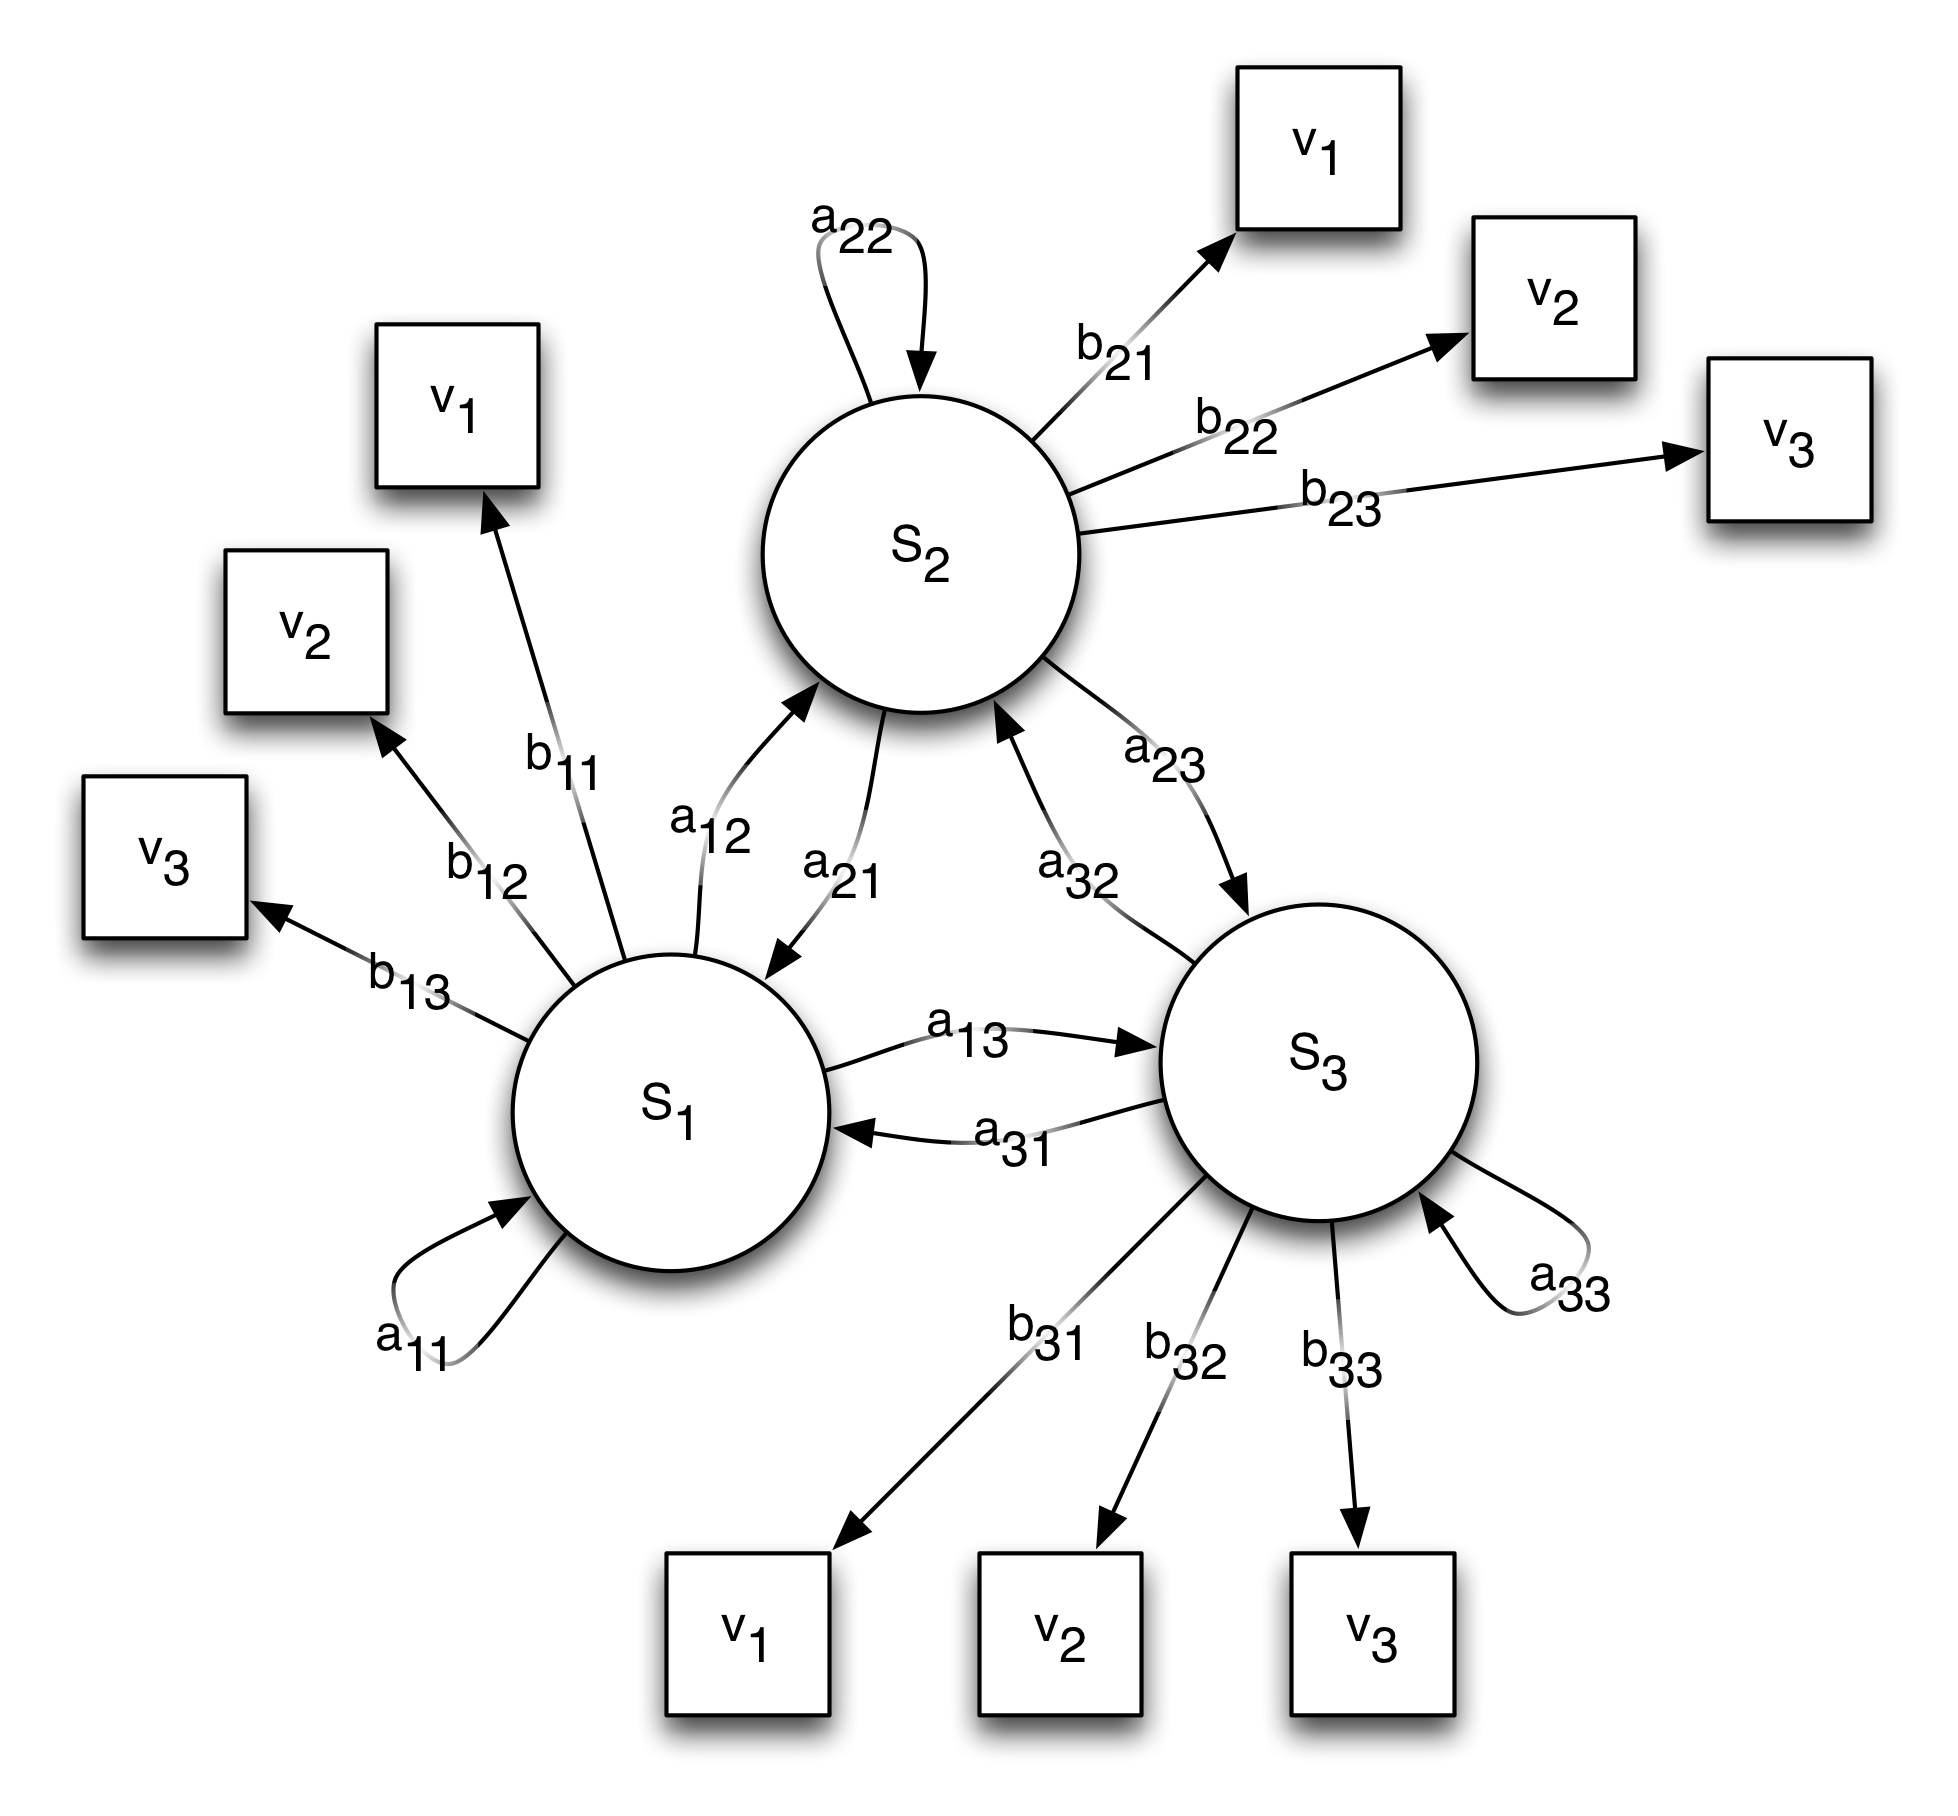
\includegraphics[width=\textwidth]{figures/hmm.png}
  \caption{HMM}
  \label{fig:hmm}
\end{figure}

Man verwendet eine HMM dann folgendermaßen: Jede Klasse $C_i$ bekommt eine HMM $\lambda_i$ deren Parameter anhand einer Stichprobe trainiert werden. Einem unbekannten Objekt, das als Folge $\mathbf{O}$ von Merkmalsvektoren beobachtet wird, wird dann die Klasse zugeordnet, für die die Wahrscheinlichkeit $P(\mathbf{O}|\lambda_i)$ (\TODO ich würde das $P_{\lambda_i}(\mathbf{O})$ schreiben...), dass die Folge von der zugehörigen HMM erzeugt wurde, maximiert wird.

\citet{Xie:2007p11427} beschreibt ein System zur Erkennung mathematischer Symbole, das auf HMM basiert. In derselben Arbeit wird auch ein Klassifizierer, der auf DTW basiert vorgestellt, und für diesen werden beeindruckende Erkennungsraten von im besten Fall 94.8 \% angeben. Obwohl sich ein Vergleich angeboten hätte werden jedoch für das HMM-basierte System keine absoluten Erkennungsraten vorgestellt, sondern lediglich relative Veränderungen, wenn mit den Parametern der HMM gespielt wird. Das stimmt etwas nachdenklich.

\citet{Winkler:1996p11716} kombiniert mehrere HMMs, die mit unterschiedlichen Merkmalen trainiert werden, und erreicht bei einem Alphabet von 84 Symbolen im besten Fall eine Erkennungsrate von 91 \%.

Von der Leistungsfähigkeit her scheinen HMMs also durchaus eine Option für Detexify zu sein. Ein Problem ergibt sich aber wieder bei der \emph{Adaptionsfähigkeit}: Die Effektivität eines HMM hängt von ihrer Modellierung ab (Anzahl der Zustände, Übergangswahrscheinlichkeiten, Ausgabewahrscheinlichkeiten) und diese müssten idealerweise für jede Symbolklasse individuell optimiert werden \cite{Fitzgerald:2005p331}. Das Hinzufügen einer neuen Symbolklasse umfasst also die Definition eines neuen HMMs und dessen Training.

\subsection{Nächste-Nachbarn-Klassifikation} \label{sub:knn}

Der $k$-nächste-Nachbarn-Algorithmus ist eines der einfachsten Verfahren um einem unbekannten Muster eine Klasse zuzuweisen. Dazu werden als Training einfach Vertreter der Klassen in einem Merkmalsraum gespeichert. Dem unbekannten Muster wird dann durch ein Mehrheitsvotum der $k$ nächsten Nachbarn eine Klasse zugeordnet. Eine zentrale Rolle nimmt dabei das Abstandsmaß, das die Nachbarschaft bestimmt, ein \cite{Jaeger:2003p1097}. Es beeinflusst die Güte der Klassifikation, aber auch durch seine Laufzeitkomplexität den zeitlichen Aufwand des Vorgangs. \TODO Literatur - Bücher?

Dabei ist KNN besonders bei Problemen beliebt, in denen die Anzahl an Klassen sehr hoch ist, wie beispielsweise bei japanischen Schriftzeichen \cite{Jaeger:2003p1097}. Eine Analyse zur Eignung für Detexify scheint also angebracht.
\TODO Laut Jiang Script Kapitel 4 ist KNN mit vielen Trainingsdaten nahezu so gut wie Bayes (optimal)
\TODO weitere Argumente für KNN: gleicht Schreibstile aus wenn genug Muster
% \citet{Tappert:1990p10302} sagt bei Online-Erkennung reichen wegen der Interaktivität einfachere Methoden, was bei mir ja voll zutrifft.

Die Bedingung der \emph{Adaptionsfähigkeit}, die ich in \ref{sec:klassifizierung} gefordert hatte, die bei den bisher vorgestellten Verfahren schwierig umzusetzen war, ist dabei bei der Nächste-Nachbarn-Klassifikation auf natürliche Weise dadurch gegeben, dass neue Trainingsmuster einfach nur gespeichert werden müssen. \emph{Interaktivität} kann leicht realisiert werden, indem jeder Klasse ein auf dem Abstandsmaß basierender Wert zugewiesen wird. So erhält man für ein unbekanntes Muster eine Rangfolge der Klassen.

Es ist also zu klären, ob es ein Abstandsmaß gibt, das die Bedingungen \emph{Skalierbarkeit} und \emph{Laufzeitkomplexität} miteinander vereinen kann.

\subsection[DTW]{DTW - Dynamic time warping} \label{sub:dtw}

Ein vielversprechendes Abstandsmaß wurde bereits in \ref{sub:hmm} erwähnt. Es wird \emph{dynamic time warping} oder auch \emph{elastic matching} genannt. Es wurde bereits erfolgreich für lateinische und chinesische Schriftzeihen eingesetzt \cite{Tappert:1990p10302}. \citet{Xie:2007p11427} erreicht damit für die Erkennung mathematischer Symbole eine Erkennungsrate von 94.8 \%. Auch \citet{Golubitsky:2009p2433} bemerken:
% In diesem Paper gibts auch Infos zum verwendete Datensatz. Weitere Statistiken zu Elastic matching Parametern.
\begin{quote}
  Among the distance measures used for classifying handwritten mathematical symbols, the elastic matching distance is known to be one of the most accurate.
\end{quote}

\citet{Golubitsky:2009p1842} vergleichen DTW mit einem eigenen Abstandsmaß, das zwar deutlich schneller zu berechnen ist, aber auch 1-1,5\% schlechtere Erkennungsraten liefert. \citet{Labahn:2008p10301} kombinieren DTW mit weiteren Methoden in einem System, das die handschriftliche Eingabe von Formeln in ein \ac{CAS} ermöglicht.
Auch \citet{Vuong:2010p10279} verwenden DTW % mit Steigung und Krümmung
zu Erkennung mathematischer Symbole in einer erst kürzlich veröffentlichten Arbeit zum Thema Web-basiertes CAS mit handschriftlicher Eingabe. Es ist auffällig, dass gerade aktuellere Arbeiten DTW einsetzen. Obwohl das Verfahren schon so lange bekannt ist \cite{Tappert:1982p10305}, ist es immer noch konkurrenzfähig.

Aus diesen Gründen ist die Wahl für die Klassifikation in Detexify auf DTW gefallen. Damit war die Aufgabe also den Algorithmus so zu implementieren und zu optimieren, dass die Bedingungen \emph{Skalierbarkeit} und \emph{Laufzeitkomplexität} erfüllt sind.

\section{DTW} % (fold)
\label{sec:dtw}

Im folgenden wird der klassische DTW-Algorithmus beschrieben und unterschiedliche Optimierungsmöglichkeiten werden diskutiert.

\subsection{Der klassische DTW-Algorithmus} % (fold)
\label{sub:der_klassische_dtw_algorithmus}

Seien zwei Folgen von Punkten
\begin{align}
  \label{eqn:a}
  A &= a_1, \dots, a_n \\
  \label{eqn:b}
  B &= b_1, \dots, b_m
\end{align}
in einem Raum \( S \ni a_i, b_i ~\forall~i \) und %die Menge von Abbildungen
% \begin{equation*}
%   \label{eqn:mappings}
%   F = \{f:\{1,\dots,n\} \rightarrow \{1,\dots,m\}, ~f~\text{surjektiv, monoton wachsend} \}  
% \end{equation*}
\( \delta : S\times S \rightarrow \mathbb{R}_0^+ \) eine Kostenfunktion
gegeben. In der Regel sind \(A\) und \(B\) Folgen in einem metrischen Raum z.B. \(\mathbb{R}^n\) und \(\delta\) ist eine Metrik.
Betrachten wir nun \( n\times m\)-Matrix 
\begin{equation} \label{eqn:matrix}
  M = (d_{i,j})_{i=1\dots n, j=1\dots m} ~\text{mit}~ d_{i,j} = \delta(a_i,b_j)
\end{equation}
, dann ist ein Warping-Pfad ein stetiger (im unten erläuterten Sinne) Pfad durch diese Matrix. 

\begin{align}
  W = w_0,\dots,w_K \hspace{1cm} w_l = (i,j)_l
\end{align}

$K$ ist dabei die Länge des Warping-Pfads. Die Stetigkeit des Pfads unterliegt den folgenden Bedingungen:

\begin{description}
  \item[Randbedingung] \( w_1 = (1,1) \) und \( w_K = (n,m) \). Dadurch beginnt der Warping-Pfad in der linken unteren Ecke der Matrix und endet in der rechten oberen Ecke.
  \item[Stetigkeitbedingung] Gegeben \( w_k = (i,j) \) und \( w_{k-1} = (i',j') \) so muss gelten \( i-i' \leqslant 1 \) und \( j-j' \leqslant 1 \). Dadurch sind nur Schritte zu benachbarten Zellen (auch diagonal) erlaubt.
  \item[Monotoniebedingung] Gegeben \( w_k = (i,j) \) und \( w_{k-1} = (i',j') \) so muss gelten \( i-i' \geqslant 0 \) und \( j-j' \geqslant 0 \). Dadurch werden rückwärtige Schritte (nach links oder unten) verhindert.
\end{description}

Es gibt natürlich einige Pfade die diese Bedingungen erfüllen. Nennen wir die Menge dieser Pfade
\[ \mathcal{W}=\{W~\text{ist Warping-Pfad}\} \]
dann ist der DTW-Abstand definiert durch
\begin{equation}
  \label{eqn:dtw}
  DTW(A,B) = \min_{W \in \mathcal{W}}{\frac{\sum_{i=1}^K d_{w_i}}{K}}
\end{equation}
. Dabei ist \( d_{w_i} \) das entsprechende Element der Matrix \ref{eqn:matrix}.

Diese abstrakte Definition bedeutet anschaulich, dass die Punkte in den zwei Folgen einander elastisch zugeordnet werden können, wobei es einige Beschränkungen gibt. Der erste Punkt der ersten Folge wird immer dem ersten Punkt der zweiten Folge und der letzte Punkt der ersten Folge immer dem letzten Punkt der zweiten Folge zugeordnet werden. Dazwischen müssen die Punkte zwar in der richtigen Reihenfolge bleiben und es dürfen keine übersprungen werden, aber es sind Mehrfachzuordnungen erlaubt. Gesucht wird die Zuordnung, die den Abstand minimiert. Abbildung~\ref{fig:dtw} illustriert dies.

\begin{figure}
  \centering 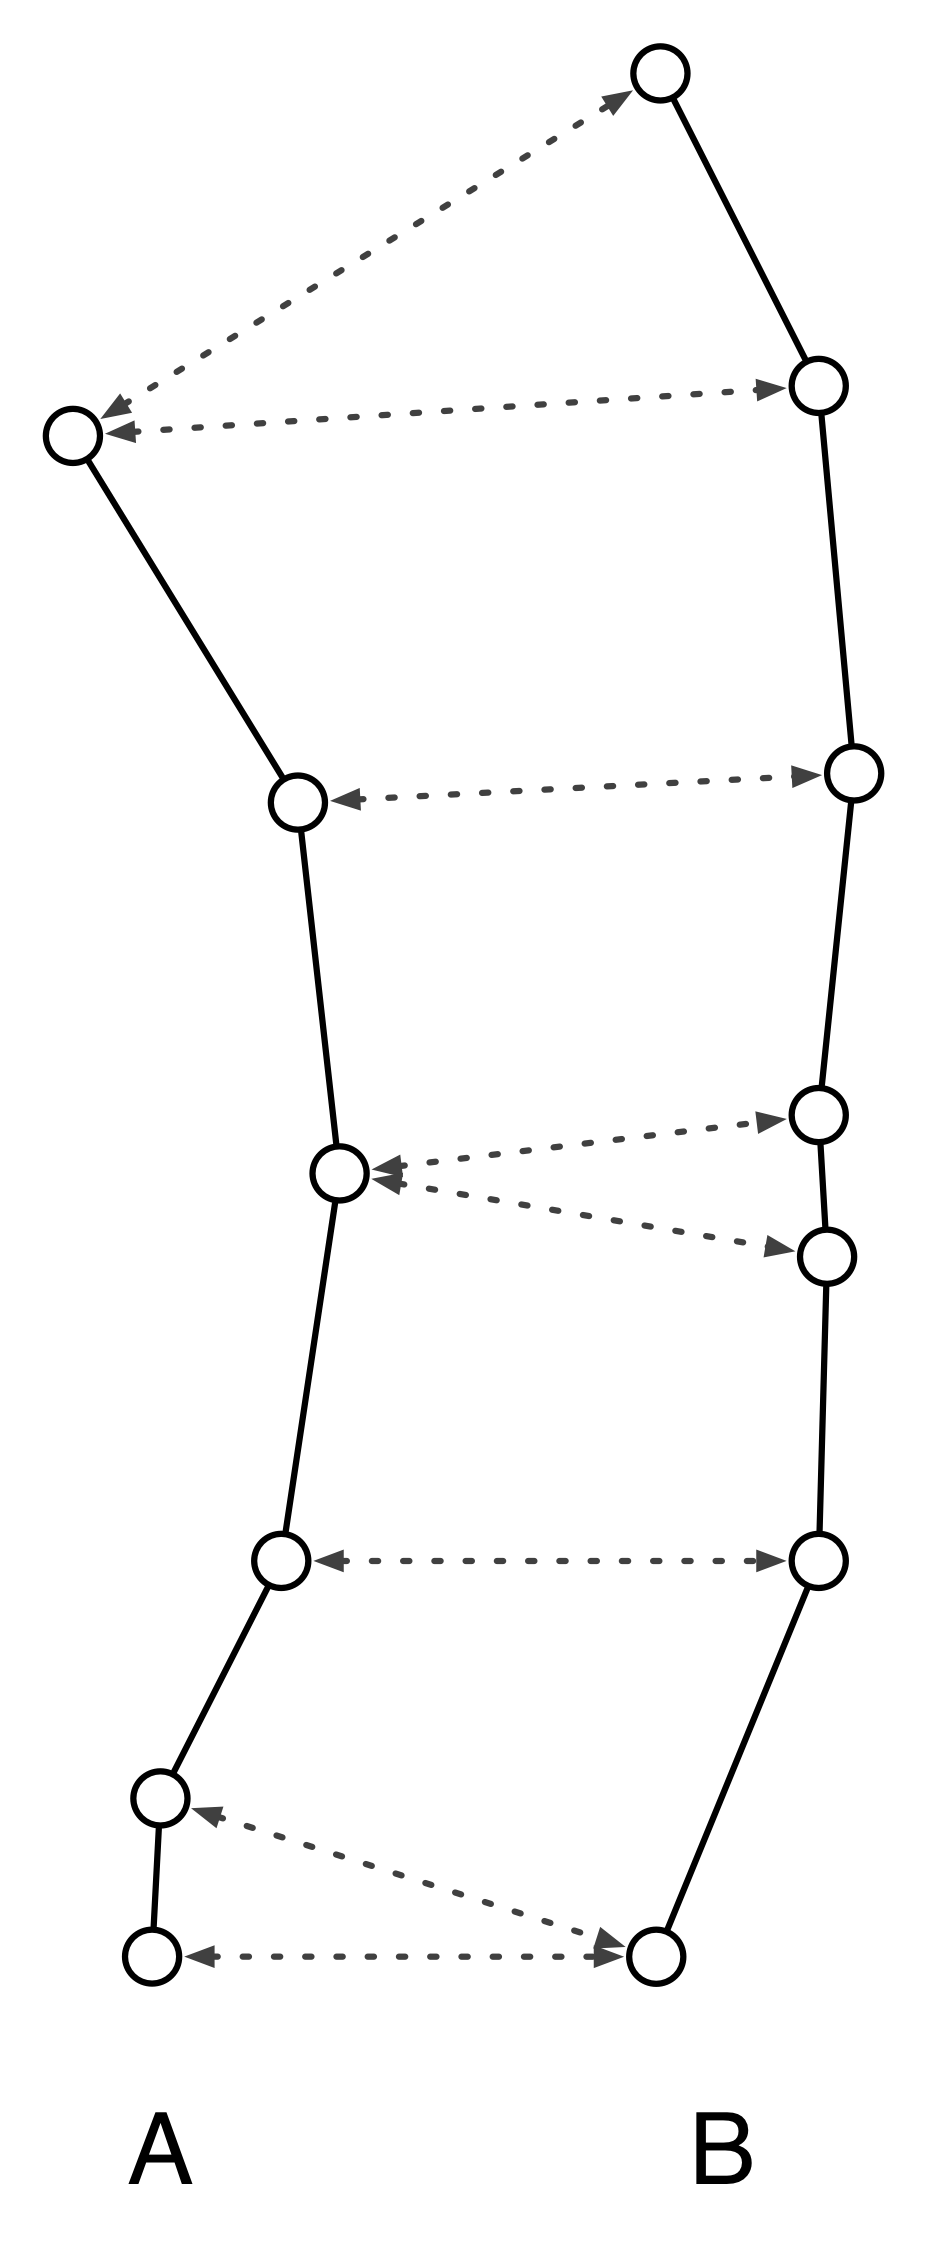
\includegraphics[width=4cm]{figures/dtw.png}
  \caption{Elastische Zuordnung bei DTW}
  \label{fig:dtw}
\end{figure}

Das gesuchte Minimum kann mithilfe von Dynamischer Programmierung gefunden werden. Gegeben die Rekurrenz
\begin{equation}
  \label{eqn:dp}
  \gamma(i,j) =
  \begin{cases}
    \sum_{k=0}^j \delta(a_0, b_k) & i = 0 \\
    \sum_{k=0}^i \delta(a_k, b_0) & j = 0 \\
    \delta(a_i,~b_j) + \min\{~\gamma(i-1,j-1),~\gamma(i-1,j),~\gamma(i,j-1)~\} & \text{sonst}
  \end{cases}  
\end{equation}

dann ist
\begin{equation}
  \label{eqn:dpdtw}
  DTW(A,B) = \frac{\gamma(n,m)}{K}
\end{equation}. \TODO Wo kommt das K her?

\TODO Dynamische Programmierung in der Literatur? z.B. Algorithmik - U Schöning - 2001

In dieser Form hat DTW die Laufzeit- und Speicherplatzkomplexität \(\mathcal{O}(nm)\). Darum wundert es nicht, dass bereits einige Wissenschaftler versucht haben, den Algorithmus zu optimieren. Auch für Detexify ist dieses Laufzeitverhalten nicht ausreichend um eine Erkennung in Echtzeit zu ermöglichen.


\subsection{Beschränkung des Warping-Pfads} % (fold)
\label{sub:constrained_warping_window}

\begin{figure}
  \centering 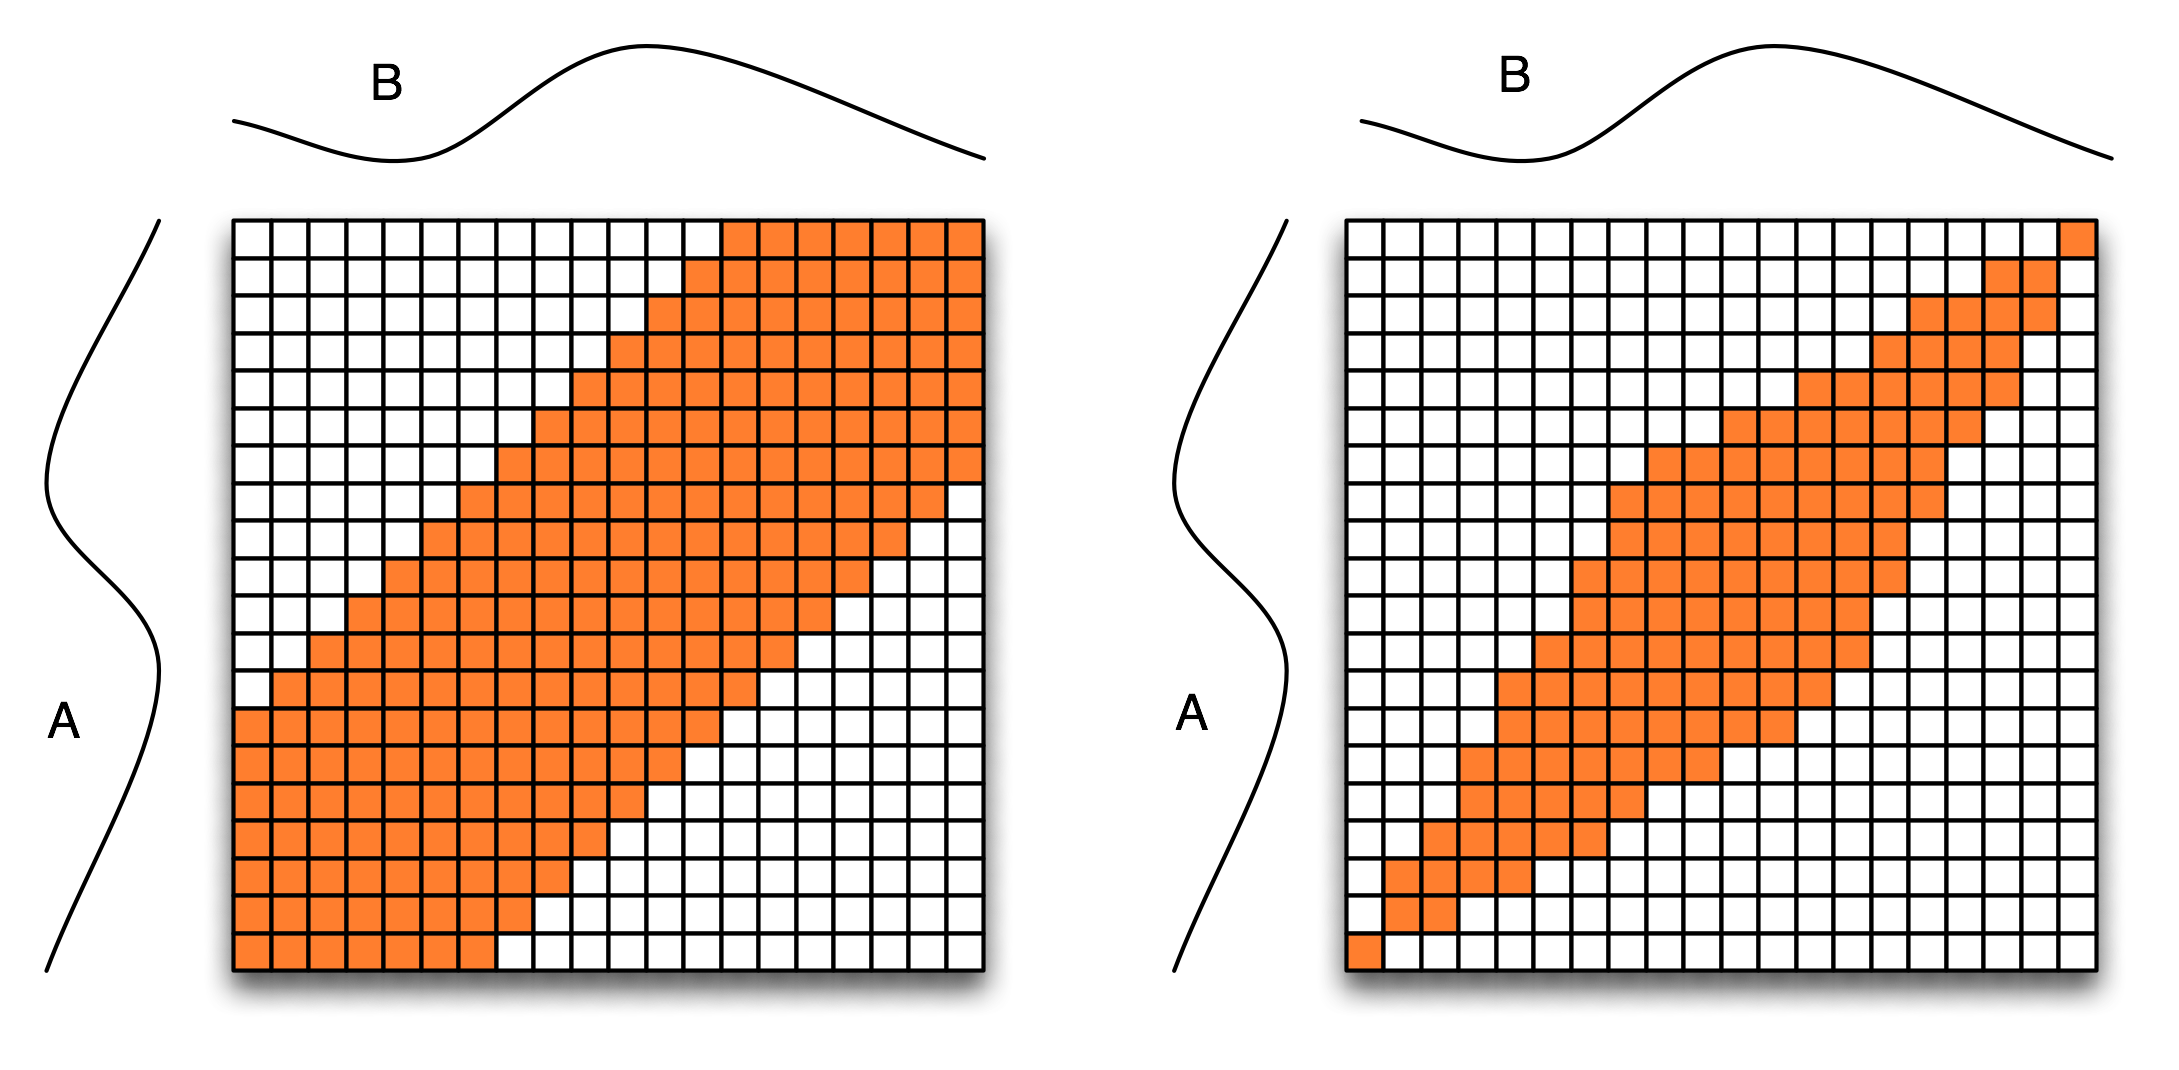
\includegraphics[width=\textwidth]{figures/constraints.png}
  \caption{Typische Beschränkungen das Warping-Pfades}
   Links: Sakoe-Chiba-Band, Rechts: Ikatura-Parallelogramm
  \label{fig:constraints}
\end{figure}


Es ist möglich DTW dadurch zu beschleunigen, dass bei der Suche nach dem optimalen Warping-Pfad nicht die ganze Matrix durchsucht wird. Stattdessen wird der Suchraum beschränkt. Abb.~\ref{fig:constraints} zeigt üblicherweise verwendete globale Beschränkungen. Es ist auch möglich lokale Beschränkungen wie in \cite{Rabiner:1993p11752} beschrieben festzulegen, \citet{Keogh:2005p7751} bemerken aber, dass das im Prinzip dasselbe, wie globale Beschränkungen sind, darum gehe ich darauf nicht näher ein. Nun könnte man glauben, dass sich eine solche Einschränkung nachteilig auswirkt. \citet{Ratanamahatana:2004p7522} berichten aber in ihrer Arbeit, dass eher das Gegenteil der Fall ist und Beschränkungen des Pfades sogar helfen, die Erkennungsraten zu verbessern. Dies kann dadurch verstanden werden, dass durch Beschränkungen pathologisches Warpen verhindert wird \cite{Keogh:2005p7751}.
%- Leichte Geschwindigkeitsverbesserung \( \mathcal{O}(ns) \) für fest gewähltes $s$
%- Sakoe and Chiba 1978 haben wohl schon rausgefunden, dass globale beschränkungen helfen \cite{Keogh:2005p7751}

Wenn beide Folgen die gleiche Länge $n$ haben, ist eine Möglichkeit den Warping-Pfad zu beschränken, einen Korridor um die Diagonale der Matrix festzulegen, aus dem nicht ausgebrochen werden darf. Beschrieben werden kann dies durch eine Beschränkung der Indizes des Warping-Pfades \( w_k = (i,j)_k \) und zwar gilt dann
\begin{equation}
  \label{eq:constraints}
  j−r(i) \leq i \leq j+r(i)
\end{equation}
, wobei $r(i)$ den erlaubten Korridor beschreibt.

Im Fall von \(r(i) = s\) also $r$ konstant reduziert sich damit die Komplexität von DTW von \( \mathcal{O}(n^2) \) auf \( \mathcal{O}(ns) \). Zusätzlich ermöglicht die Beschränkung bei fester Länge $n$ der Folgen aber eine weitere viel effektivere Optimierung:

\subsection{Untere Schranken} % (fold)
\label{sub:lower_bounding}

Gegeben ein Abstandsmaß \( \delta : S\times S \rightarrow \mathbb{R}_0^+ \) und eine untere Schranke \( \delta_{LB} \) d.h. \( \delta_{LB}(a,b) \leq \delta(a,b) ~\forall~ a,b \in S \), die deutlich günstiger zu berechnen ist, dann lässt sich mit dem folgenden naiven Algorithmus eine sequentielle Suche nach dem nächsten Nachbarn eines Elementes \( c \in S \) beschleunigen (vergl. \cite{Keogh:2005p7751}).

\begin{algorithm}
  \caption{Beschleunigung der Suche nach dem nächsten Nachbarn eines Elementes \(c\) durch eine untere Schranke}
  \begin{algorithmic}
    \STATE $\text{best\_so\_far} \gets \infty$
    \FORALL{samples $s$}
      \STATE $\text{lb\_dist} \gets \delta_{LB}(c,s)$
      \IF{$\text{lb} < \text{best\_so\_far}$}
        \STATE true\_dist $\gets \delta(c,s)$
        \IF{$\text{true\_dist} < \text{best\_so\_far}$}
          \STATE best\_so\_far $\gets$ true\_dist
          \STATE nearest\_neighbor $\gets s$
        \ENDIF
      \ENDIF
    \ENDFOR
  \end{algorithmic}
\end{algorithm}

Für DTW für Folgen derselben Länge $n$ mit reellen Messpunkten mit einer Beschränkung des Warping-Pfades der Form \ref{eq:constraints} haben \citet{Keogh:2005p7751} eine scharfe untere Schranke angegeben. Zudem haben \citet{Ratanamahatana:2004p7522} die Kritik entkräftet, dass vor der Verwendung einer solchen Optimierung eine lineare Interpolation der Folgen nötig ist, um sie auf dieselbe Länge zu bringen, und damit der Vorteil Folgen unterschiedlicher Länge vergleichen zu können verlogen ginge. Eine untere Schranke scheint also eine reizvolle Möglichkeit zu sein DTW zu beschleunigen.

\TODO wer hat vor \citet{Keogh:2005p7751} untere Schranken angegeben? Muss ich das erwähnen?

In Fall von Detexify sind die einzelnen Punkte der Folgen aber Punkte im \( \mathbb{R}^2 \) (siehe \ref{sec:vorverarbeitung}) und es ist intuitiv einzusehen, dass eine Reduktion auf eine Dimension einen zu hohen Informationsverlust nach sich ziehen würde. Es ist zwar möglich auf eine zu \cite{Keogh:2005p7751} analoge Weise eine untere Schranke zu definieren, und das werde ich als nächstes tun - es zeigt sich jedoch, dass diese untere Schranke keine vorteilhaften Laufzeiteigenschaften mehr hat. Darum wird auch der formale Beweis, dass es sich wirklich um eine untere Schranke handelt übergangen.

\subsection{Eine untere Schranke für DTW für Folgen im \( \mathbb{R}^2 \)}

\subsubsection{LB\_Keogh}
\label{ssub:lb_keogh}

Bevor ich meine untere Schranke erläutere, gebe ich noch eine kurze Erklärung der von \citet{Keogh:2005p7751} definierten unteren Schranke LB\_Keogh an.

Seien
\begin{align}
  Q &= q_1 \dots q_n  & q_i \in \mathbb{R} \\
  C &= c_1 \dots c_n  & c_i \in \mathbb{R}
\end{align}
zwei Folgen gleicher Länge $n$. \( \mathcal{W}_r \) sei die Menge der durch \(r\) beschränkten Warping-Pfade (siehe \ref{eq:constraints}). DTW sei (leicht verändert) gegeben durch
\begin{equation}
  \label{eq:keoghdtw}
  DTW(Q,C) = \min_{W \in \mathcal{W}_r}{\sqrt{\sum_{i=1}^n d_{w_i}}}
\end{equation}.
Mithilfe von \(r\) werden nun weitere Folgen $U$ und $L$ definiert:
\begin{align}
  U_i &= \max ~\{ q_{i-r}, \dots, q_{i+r} \}\\
  L_i &= \min ~\{ q_{i-r}, \dots, q_{i+r} \}
\end{align}
Es gilt offensichtlich
\begin{equation}
  \forall ~ i ~ U_i \geq q_i \geq L_i
\end{equation}.
Nun können wir eine untere Schranke für \ref{eq:keoghdtw} wiefolgt definieren:
\begin{equation}
  \label{eq:lbkeogh}
  \operatorname{LB\_Keogh}(Q,C) = \sqrt{\sum_{i=1}^n
  \begin{cases}
    \delta(c_i, U_i) & c_i > U_i \\
    \delta(c_i, L_i) & c_i < L_i \\
    0 & \text{sonst}
  \end{cases}  
  }
\end{equation}

Die Intuition dahinter ist die folgende. Die Folgen $U$ und $L$ bilden eine Hülle um die ursprüngliche Folge $Q$. LB\_Keogh ist dann sozusagen der Abstand einer neuen Folge $C$ zu dieser Hülle (siehe Abbildung \ref{fig:lb_keogh}). Dass dies tatsächlich eine untere Schranke ist, haben \citet{Keogh:2005p7751} gezeigt. Sie argumentieren auch, dass ihre Schranke schärfer also die bisher in der Literatur aufgetauchten ist.

\begin{figure}
  \centering 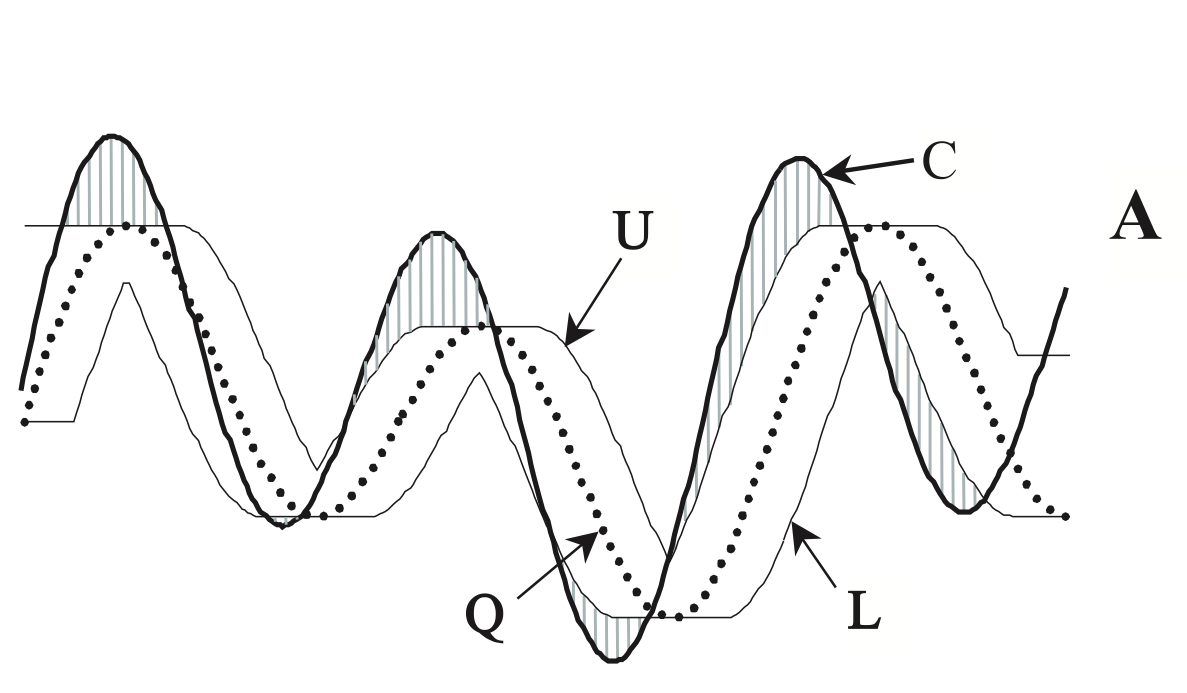
\includegraphics[width=10cm]{figures/lb-keogh.png}
  \caption{Grafische Darfstellung von LB\_Keogh. Grafik entnommen aus \cite{Keogh:2005p7751}}
  \label{fig:lb_keogh}
\end{figure}

\subsubsection{\(\mathbb{R}^2\)-analog zu LB\_Keogh}\label{subs:lb_keogh_analog}

Es ist möglich für zwei Folgen 
\begin{align}
  A &= a_1 \dots a_n  & a_i \in \mathbb{R}^2 \\
  B &= b_1 \dots b_n  & b_i \in \mathbb{R}^2
\end{align}
auf analoge Weise eine untere Schranke zu definieren. \( \mathcal{W}_r \) sei wieder die Menge der durch \(r\) beschränkten Warping-Pfade. Wir definieren dann eine neue Folge $C$ durch
\begin{equation}
  C_i = \operatorname{conv} ~\{ a_{i-r}, \dots, a_{i+r} \}
\end{equation}
wobei
\[
  \operatorname{conv} X = \bigcap_{X\subseteq K \subseteq V \atop K\ \mathrm{konvex}} K
\]
die konvexe Hülle ist. Die neue Folge $C$ besteht also aus konvexen Polygonen. Für \ref{eq:keoghdtw} lässt sich nun eine untere Schranke wiefolgt definieren:
\begin{equation}
  \label{eq:lbkeoghanalog}
  \operatorname{LB}(A,B) = \sqrt{\sum_{i=1}^n
  \begin{cases}
    0 & b_i \in C_i \\
    \delta(b_i, C_i) & \text{sonst}
  \end{cases}  
  }
\end{equation}
und dabei ist natürlich \( \delta(b_i, C_i) = \min\limits_{c \in C_i} \delta(b_i, c) \).

\FIXME Ich habe gerade den Verdacht, dass das gar nicht stimmt... ich darf bloß den Abstand zu den Ecken nehmen. Die Anzahl der Ecken ist kleiner gleich $r$ aber ich brauche immer noch im worst case $r$ Vergleiche womit LB also \( \mathcal{O}(rn) \) ist, also nicht schneller als der ursprüngliche Algorithmus. Passt auch mit dem zusammen, was ich hier sagen will, aber ich muss wohl anders argumentieren...

% subsubsection lower_bounding (end)

\subsection{Greedy Matching} % (fold)
\label{sec:greedy}

Es ist möglich DTW mit einem Greedy-Algorithmus zu approximieren.
\TODO Allgemeines zu Greedy-Algorithmen (unterschiede zu Dynamischer Programmierung (nicht-erschöpfend)) z.B. Algorithmik - U Schöning - 2001

Grundsätzlich funktioniert eine Greedy-Approximation von DTW bei zwei Folgen $A$ und $B$ mit \(a_i,b_i \in S\) und einem Abstandsmaß \(\delta:S\times S \rightarrow \mathbb{R}_0^+\) folgendermaßen. Beginne mit den Startpunkten $a_1$ und $b_1$ ordne diese einander zu. Ordne dann jeweils die nächsten Punkte so einander zu, dass der Abstand unter \(\delta\) minimal ist (wähle das lokale Optimum). Wiederhole dies, bis in einer der beiden Folgen nur noch ein Punkt übrig ist. Ordne alle restlichen Punkte der anderen Folge diesem zu. Algorithmus \ref{alg:greedy} zeigt eine Implementierung in Pseudocode.
Wie man sieht hat der Algorithmus einen konstanten Speicherplatzaufwand und eine lineare Laufzeit.
% hier schon haskell-implementierung erwähnen?

\begin{algorithm}
  \caption{Greedy Matching}
  \label{alg:greedy}
  \begin{algorithmic}
    \STATE $a \gets \text{next from}~A$
    \STATE $b \gets \text{next from}~B$
    \STATE $d \gets \delta(a,b)$
    \STATE $a' \gets \text{next from}~A$
    \STATE $b' \gets \text{next from}~B$
    \WHILE{points left in $A$ $\wedge$ points left in $B$}
      \STATE $l, m, r \gets \delta(a',b), \delta(a', b'), \delta(a, b')$
      \STATE $\mu \gets \min ~\{l, m, r\}$
      %\COMMENT{ Important line }
      \STATE $d \gets d + \mu$
      \IF{$l = \mu$}
        \STATE $a \gets a'$
        \STATE $a' \gets \text{next from}~A$
      \ELSIF{$r = \mu$}
        \STATE $b \gets b'$
        \STATE $b' \gets \text{next from}~B$
      \ELSE
        \STATE $a \gets a'$
        \STATE $b \gets b'$
        \STATE $a' \gets \text{next from}~A$
        \STATE $b' \gets \text{next from}~B$
      \ENDIF
    \ENDWHILE
    \IF{no points left in $A$}
      \FORALL{points $p$ in $B$}
        \STATE $d \gets d + \delta(a',p)$
      \ENDFOR
    \ELSIF{no points left in $B$}
      \FORALL{points $p$ in $A$}
        \STATE $d \gets d + \delta(b',p)$
      \ENDFOR
    \ENDIF
  \end{algorithmic}
\end{algorithm}

%\lstinputlisting[language=Haskell,firstline=43,lastline=56]{../../code/hs-classifier/DTW.hs}

\citet{MacLean:2010p9970} stellen eine Variante dieses Algorithmus vor. Sie verwenden ihn zur Erkennung mathematischer Symbole in Mathbrush, das in dieser Arbeit bereits erwähnt wurde (siehe auch \ref{sub:mathbrush} und \cite{Labahn:2008p10301}). Sie gehen bei der Zuordnung von Punkten aber simultan von beiden Seiten vor.
Welche Vorteile das gegenüber einer einseitigen Strategie bringt, erklären sie nicht. Sie vergleichen ihren Greedy-Algorithmus jedoch mit dem Standard-DTW-Algorithmus und kommen zum Ergebnis, dass der Greedy-Algorithmus zur Unterscheidung von mathematischen Symbolen ebenso geeignet ist. Insbesondere bei einer kleinen Anzahl von Punkten pro Strich (<30) ist der Greedy-Algorithmus sogar gleich gut geeignet und durch seine lineare Laufzeit natürlich wesentlich schneller. Bei ihren Tests verwenden sie 15796 handgeschriebene Symbole aus 70 Symbolklassen geschrieben von 20 unterschiedlichen Personen.

\subsection{Elimination}
\label{sec:elimnimation}

Möglich Suche durch Elimination irrelevanter Trainingsmuster zu beschleunigen...
\cite{Watt:2005p1816} schlägt Elimination durch klassische features vor
\TODO da DTW keine Metrik ist können klassische Eliminationsverfahren wie der Voronoi-Trick nicht angewandt werden also keine exakte Lösung. Vielleicht trotzdem mal Greedy-Algorithmus nach Hart (siehe Jiang-Script) testen?

\TODO Voronoi-Trick und Greedy-Hart in der Literatur?

\subsection{Parameter}
\label{sec:parameter}

Die unterschiedlichen Varianten von DTW können durch unterschedliche Parameterwahlen beeinflusst werden.
n - Anzahl Punkte im Striche
r - Fensterbreite bei beschränktem DTW
Verwendetes inneres Abstandsmaß (Manhatten/Euklidisch/Mit Steigung und Krümmung \citet{Vuong:2010p10279})

\citet{Golubitsky:2009p1842} enthält ganz viele Statistiken zu Parametern für DTW (und Vergleich mit Funktionalapproximationsmaß)
\begin{itemize}
  \item k (Anzahl der Nachbarn)
  \item Anzahl der Punkte
\end{itemize}


% eigentlich egal: siehe \cite{Vuong:2010p10279} Natural Log, symbol recognition is implemented using a statistical approach based on Gaussian Density Estimation \dots siehe auch \cite{Vuong:2010p10279} \TODO Paper suchen


%!TEX root = /Users/daniel/Documents/thesis/thesis.tex
\chapter{Benchmarks} % (fold)
\label{cha:benchmarks}

\TODO Optimierung von

\begin{description}
  \item[$n$] - Anzahl der Punkte pro Strich
  \item[$\delta$] - das verwendete innere Abstandsmaß (siehe \ref{sub:dtw})
  \item[$C$] - Anzahl der Trainingsmuster pro Klasse
  \item[$\alpha$] - Grenzwinkel für dominante Punkte
\end{description}

- sozusagen $k=1$ aber wir ranken ja eh, von daher nicht so relevant

- Folgen erst mal \citet{Golubitsky:2009p1842} mit $n=25$.

- Testen für $\delta$ euklidische Metrik und Manhattan-Metrik ~> Manhattan ist doch tatsächlich besser.

- Finden heraus, dass gdtw nahezu so gut ist wie dtw also schauen verwenden wir cdtw gar nicht da der Performancegewinn ohnehin nicht groß wäre also entfällt Optimierung von $r$

- Beginnen mit $C=50$ - andere Werte dann experimentell

\section{Kleiner Datensatz}
\label{sec:kleiner_datensatz}

In diesem Abschnitt werden mithilfe eines Teils der verfügbaren Trainingsdaten die Verfahren auf ihre Güte überprüft und die Parameter optimiert. Der kleine Datensatz besteht aus 100 zufällig aus der Datenbank ausgewählten Symbolen.
Es wurden 75 Muster pro Symbolklassen zufällig ausgewählt wovon 50 für das Training und 50 als Testmuster verwendet wurden. Dies ergibt 2500 Tests.

Folgende Symbole werden verwendet:
$\$$,
$\{$,
$\copyright$,
$\}$,
$\S$,
$\&$,
$\#$,
$\%$,
$\checkmark$,
\aa,
\AA,
\ae,
\DH,
\DJ,
$\EUR$,
$\cup$,
$\oplus$,
$\times$,
$\ast$,
$\otimes$,
$\pm$,
$\cap$,
$\vee$,
$\cdot$,
$\odot$,
$\wedge$,
$\circ$,
$\bigotimes$,
$\prod$,
$\sum$,
$\bigodot$,
$\int$,
$\oint$,
$\approx$,
$\equiv$,
$\perp$,
$\cong$,
$\propto$,
$\vdash$,
$\sim$,
$\simeq$,
$\therefore$,
$\because$,
$\subseteq$,
$\geq$,
$\leq$,
$\ll$,
$\neq$,
$\lesssim$,
$\gtrsim$,
$\triangleq$,
$\Rightarrow$,
$\rightarrow$,
$\Leftrightarrow$,
$\mapsto$,
$\alpha$,
$\theta$,
$\tau$,
$\beta$,
$\vartheta$,
$\pi$,
$\gamma$,
$\phi$,
$\delta$,
$\rho$,
$\varphi$,
$\epsilon$,
$\lambda$,
$\chi$,
$\varepsilon$,
$\mu$,
$\sigma$,
$\psi$,
$\zeta$,
$\nu$,
$\omega$,
$\eta$,
$\xi$,
$\Gamma$,
$\Lambda$,
$\Sigma$,
$\Psi$,
$\Delta$,
$\Xi$,
$\Omega$,
$\Theta$,
$\Pi$,
$\Phi$,
$\bot$,
$\forall$,
$\ell$,
$\hbar$,
$\in$,
$\not\in$,
$\partial$,
$\exists$,
$[$,
$/$,
$\aleph$,
$\infty$

Davon sind manche, wie $\odot$ (\verb!\odot!) und $\bigodot$ (\verb!\bigodot!) oder $\sum$(\verb!\sum!) und $\Sigma$~(\verb!\Sigma!) eigentlich dieselben Symbole. Es wurden aber keine Maßnahmen ergriffen, um solche Zweideutigkeiten aufzuheben, da durch die Interaktivität der Anwendung ohnehin in erste Linie eine hohe Top 5-Erkennungsrate wichtig ist.

\subsection{Gierig oder nicht?}
\label{sub:gierig_oder_nicht}

\begin{itemize}
  \item $C=50$
  \item $\delta\sim\text{Euklid}$
  \item $n=25$ (optimal nach \citet{Golubitsky:2009p1842})
\end{itemize}

Striche werden einfach konkateniert. $DTW (DTW euklid) a b$ auch denkbar, ist aber langsamer und schneidet schlechter ab (in kleineren Benchmarks ermittelt). Abbildung \ref{chart:dtw-vs-gdtw} zeigt, dass Greedy kaum schlechter was die Ergebnisse von \citet{MacLean:2010p9970} bestätigt.

\begin{figure}[htbp]
  \begin{center}
    \includegraphics[width=\textwidth]{charts/dtw-vs-gdtw.pdf}
  \end{center}
  \caption{Greedy DTW gegen klassisches DTW}
  \label{chart:dtw-vs-gdtw}
\end{figure}

\begin{figure}[htbp]
  \begin{center}
    \includegraphics[width=.75\textwidth]{charts/dtw-vs-gdtw-ms.pdf}
  \end{center}
  \caption{Greedy DTW gegen klassisches DTW - Laufzeit}
  \label{chart:dtw-vs-gdtw-ms}
\end{figure}

% chapter benchmarks (end)

\subsection{Inneres Abstandsmaß} % (fold)
\label{sub:inneres_abstandsmaß}
Euklid gegen Manhattan $\delta$
Abbildung \ref{chart:dtw-vs-gdtw} zeigt, dass die günstigere Manhattan-Metrik sogar besser ist.
% subsection inneres_abstandsmaß (end)

\subsection{Anzahl Trainingsmuster} % (fold)
\label{sub:anzahl_trainingsmuster}

\begin{figure}[htbp]
  \begin{center}
    \includegraphics[width=.75\textwidth]{charts/samples.pdf}
  \end{center}
  \caption{Einfluss der Anzahl der Trainingsmuster $C$}
  \label{chart:samples}
\end{figure}

- Klassifizierungsserver verwirft alte Trainingsmuster, wenn $C$ überschritten
Lorem ipsum dolor sit amet, consectetur adipisicing elit, sed do eiusmod tempor incididunt ut labore et dolore magna aliqua. Ut enim ad minim veniam, quis nostrud exercitation ullamco laboris nisi ut aliquip ex ea commodo consequat. Duis aute irure dolor in reprehenderit in voluptate velit esse cillum dolore eu fugiat nulla pariatur. Excepteur sint occaecat cupidatat non proident, sunt in culpa qui officia deserunt mollit anim id est laborum.
% subsection anzahl_klassen (end)

\subsection{Anzahl Punkte pro Strich} % (fold)
\label{sub:anzahl_punkte_pro_strich}

\begin{figure}[htbp]
  \begin{center}
    \includegraphics[width=.75\textwidth]{charts/points.pdf}
  \end{center}
  \caption{Einfluss der Anzahl der Punkte pro Strich $n$}
  \label{chart:points}
\end{figure}

Lorem ipsum dolor sit amet, consectetur adipisicing elit, sed do eiusmod tempor incididunt ut labore et dolore magna aliqua. Ut enim ad minim veniam, quis nostrud exercitation ullamco laboris nisi ut aliquip ex ea commodo consequat. Duis aute irure dolor in reprehenderit in voluptate velit esse cillum dolore eu fugiat nulla pariatur. Excepteur sint occaecat cupidatat non proident, sunt in culpa qui officia deserunt mollit anim id est laborum.
% subsection anzahl_punkte_pro_strich (end)

\subsection{Dominante Punkte} % (fold)
\label{sub:dominante_punkte}

\begin{figure}[htbp]
  \begin{center}
    \includegraphics[width=.75\textwidth]{charts/degree.pdf}
  \end{center}
  \caption{Einfluss des Winkels $\alpha$}
  \label{chart:degree}
\end{figure}

Lorem ipsum dolor sit amet, consectetur adipisicing elit, sed do eiusmod tempor incididunt ut labore et dolore magna aliqua. Ut enim ad minim veniam, quis nostrud exercitation ullamco laboris nisi ut aliquip ex ea commodo consequat. Duis aute irure dolor in reprehenderit in voluptate velit esse cillum dolore eu fugiat nulla pariatur. Excepteur sint occaecat cupidatat non proident, sunt in culpa qui officia deserunt mollit anim id est laborum.
% subsection dominante_punkte (end)

\section{Großer Datensatz}
\label{sec:kleiner_datensatz}


627 Symbole (die mit mind 15 Trainingsmustern) pro Klasse max 100 Trainingsmuster davon ein drittel als Testmuster und der Rest Training
13411 Testmuster
27460 Trainingsmuster
%!TEX root = /Users/daniel/Documents/thesis/thesis.tex
\chapter{Zusammenfassung und Ausblick}

\TODO

\begin{itemize}
  \item Vergleich verschiedener innerer Maße
  \item Kombination von Klassifizierern
  \item Version, die ohne Web auskommt
  \item \dots
\end{itemize}

\appendix
%!TEX root = /Users/daniel/Documents/thesis/thesis.tex
\chapter{Nutzungsstatistiken} % (fold)
\label{cha:nutzungsstatistiken}

Dieses Kapitel enthält einige Graphen, die Aufschluss über die Benutzer von Detexify geben können. Die Daten stammen aus dem Zeitraum vom 22.8.2010 bis zum 21.9.2010. Die Nutzungsdaten werden permanent mithilfe von Google Analytics \cite{analytics} gesammelt. Ich gebe keine Interpretation der Daten an. Dem Leser steht frei seine eigenen Schlüsse zu ziehen.

\begin{figure}[htbp]
  \begin{center}
    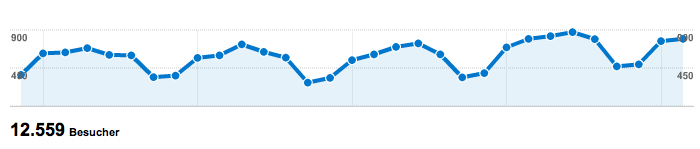
\includegraphics[width=.75\textwidth]{usage/users.png}
  \end{center}
  \caption{Besucherzahlen innerhalb eines Monats. Es ist klar ein Wochenrhythmus erkennbar.}
\end{figure}

\begin{figure}[htbp]
  \begin{center}
    \includegraphics[width=\textwidth]{usage/os.pdf}
  \end{center}
  \caption{Betriebssysteme der Nutzer}
\end{figure}

\begin{figure}[htbp]
  \begin{center}
    \includegraphics[width=\textwidth]{usage/browser.pdf}
  \end{center}
  \caption{Webbrowser der Nutzer}
\end{figure}

\begin{figure}[htbp]
  \begin{center}
    \includegraphics[width=\textwidth]{usage/country.pdf}
  \end{center}
  \caption{Länder}
\end{figure}

\begin{figure}[htbp]
  \begin{center}
    \includegraphics[width=.75\textwidth]{usage/city.pdf}
  \end{center}
  \caption{Städte}
\end{figure}

\begin{figure}[htbp]
  \begin{center}
    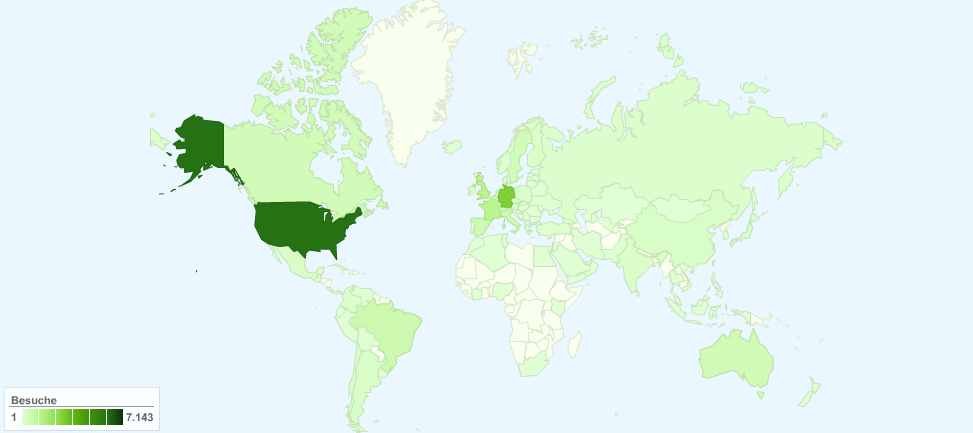
\includegraphics[width=\textwidth]{usage/countrymap.png}
  \end{center}
  \caption{Karte der Zugriffe: Länder}
\end{figure}

\begin{figure}[htbp]
  \begin{center}
    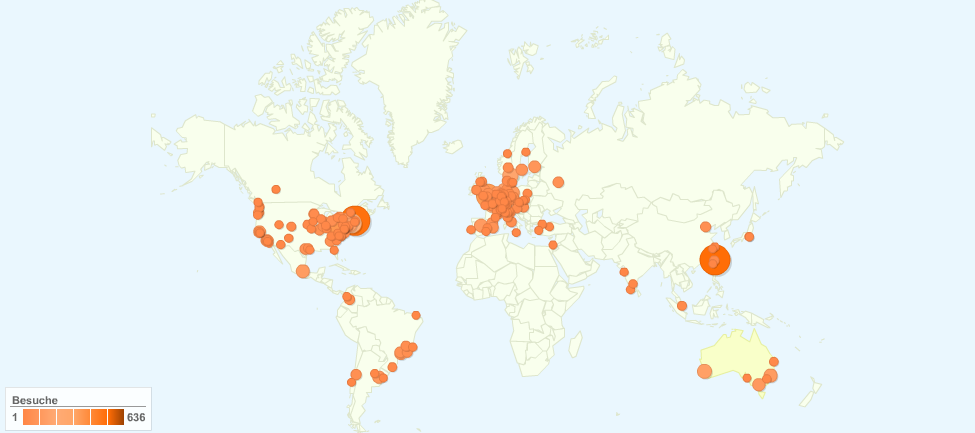
\includegraphics[width=\textwidth]{usage/citymap.png}
  \end{center}
  \caption{Karte der Zugriffe: Städte}
\end{figure}


% chapter nutzungsstatistiken (end)

%!TEX root = /Users/daniel/Documents/thesis/thesis.tex
\chapter{Abkürzungen}

% Acronyme
\begin{acronym}[YTM]
\setlength{\itemsep}{-\parsep}
\acro{API}{Application Programming Interface}
\acro{CAS}{Computer Algebra System}
\acro{WYSIWYG}{What You See Is What You Get}
\acro{WYSIWYM}{What You See Is What You Mean}
\acro{HTML}{Hyper Text Markup Language}
\acro{URL}{Uniform Resource Locator}
\acro{URI}{Uniform Resource Identifier}
\acro{HATEOAS}{Hypermedia as the Engine of Application State}
\acro{REST}{Representational State Transfer}
\acro{HTTP}{Hypertext Transfer Protocol}
\acro{JSON}{Javascript Object Notation}
\acro{SVG}{Scalable Vector Graphics}
\acro{betai}[$\beta_i$]{Regressionskoeffizient}
\acro{SVM}{Support Vector Machines}
\acro{DAGSVM}{directed acyclic graph-SVM}
\acro{WTA}{Winner-takes-all}
\acro{MWV}{Max-wins voting}
\acro{HMM}{Hidden Markov Model}
\acro{NN}{Neuronale Netze}
\acro{k-NN}{k-nearest neighbor}
\acro{DTW}{dynamic time warping}
\acro{GDTW}{greedy dynamic time warping}
\end{acronym}

%!TEX root = /Users/daniel/Documents/thesis/thesis.tex
\chapter{Benutzerhandbuch} % (fold)
\label{man:benutzerhandbuch}

In diesem Kapitel wird die Benutzung von Detexify erläutert. Die Anwendung wird aufgerufen indem man Adresse \url{http://detexify.kirelabs.org} besucht.

\section{Symbolssuche} % (fold)
\label{man:symbolsuche}

Die erste Ansicht, nachdem man die Anwendung aufgerufen hat, ist die Symbolsuche. Der schwarz umrahmte quadratische Bereich mit dem Hinweis \textbf{\texttt{Draw here!}} ist die Zeichenfläche. Auf dieser kann ein Symbol gezeichnet werden und nach jedem abgeschlossenen Strich beginnt der Erkennungsvorgang\marginline{\textsf{\textbf{Erkennung}}}. Ein Indikator in der rechten unteren Ecke der Zeichenfläche weist auf einen aktiven Erkennungsvorgang hin. Währenddessen können weitere Striche auf die Zeichenfläche gezeichnet werden. Mit einen Klick auf \textbf{\texttt{clear}} in der unteren linken Ecke der Zeichenfläche kann der Erkennungsvorgang abgebrochen werden und der Inhalt der Zeichenfläche wird gelöscht.

Ist der Erkennungsvorgang abgeschlossen, so erscheint rechts neben der Zeichenfläche die Ergebnisliste\marginline{\textsf{\textbf{Ergebnisliste}}}. Diese enthält für jedes Ergebnis eine Grafik des Symbols, den Befehl und gegebenenfalls das Paket, das benötigt wird. Es werden zuerst nur die besten fünf Ergebnisse angezeigt. Am unteren Ende der Ergebnisliste kann mit einem Klick die vollständige Ergebnisliste angezeigt werden.

Nun kann noch mit einen Klick auf die Grafik eines Ergebnisses das entsprechende Symbol mit der aktuellen Zeichnung trainiert werden.\marginline{\textsf{\textbf{Training}}}

Oberhalb der Zeichenfläche befindet sich die Navigationsleiste.\marginline{\textsf{\textbf{Navigation}}} Über diese kann man zur Symboltabelle gelangen.

% section ein_symbol_suchen (end)

\section{Symbolstabelle} % (fold)
\label{man:symboltabelle}

Über den Besuch der Adresse \url{http://detexify.kirelabs.org/symbols.html} oder über die Navigationsleiste durch einen Klick auf \textbf{\texttt{symbols}}. Die Symboltabelle befindet sich auf der linken Seite der Ansicht und ähnelt der Ergebnisliste bei der Symbolsuche.

Am oberen Rand der Tabelle befinden sich Bedienelemente, die es ermöglichen die Symboltabelle nach Befehlen oder Paketen zu filtern\marginline{\textsf{\textbf{Filter}}}. Dazu muss der gewünschte Filter ausgewählt werden und eine beliebige Zeichenfolge, nach der gefiltert werden soll, in das vorhandene Textfeld eingegeben werden.

Klickt man auf einen Eintrag der Symboltabelle, so öffnet sich unterhalb dieses Eintrags eine Zeichenfläche. Auf diese kann dann das Symbol gezeichnet werden und mit einem Klick auf \textbf{\texttt{train}}\marginline{\textsf{\textbf{Training}}} am unteren linken Rand der Zeichenfläche wird das Symbol mit der Zeichnung trainiert. Die Zeichnung kann auch ohne das Symbol zu trainieren wieder gelöscht werden, indem daneben auf \textbf{\texttt{cancel}} geklickt wird.

Oberhalb der Filterkontrollen befindet sich wieder die Navigationsleiste.\marginline{\textsf{\textbf{Navigation}}} Über diese kann man durch einen Klick auf \textbf{\texttt{classify}} zurück zur Symbolsuche gelangen.

% subsection training (end)

% section ein_symbol_trainieren (end)

% chapter benutzerhandbuch (end)
\chapter{Kunst}
\label{cha:kunst}

Da das Training von Detexify komplett von den Nutzern übernommen wird (siehe \ref{sec:crowdsourcing}) und nicht überwacht wird, sammeln sich in der Datenbank mit Trainingsbeispielen allerlei Zeichnungen an, die mit dem Symbol, für das sie gespeichert wurden nichts zu tun haben. Die interessantesten davon sind in der folgenden Übersicht aufgelistet. Dies dient einzig und allein der Belustigung des Lesers.



\includegraphics[width=0.2\textwidth]{art/Safari.png}
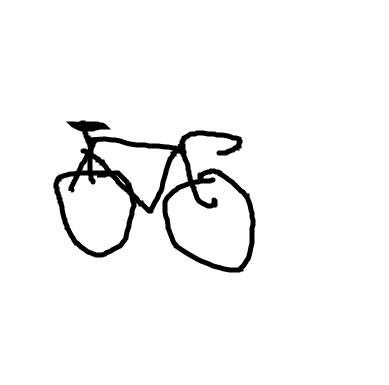
\includegraphics[width=0.2\textwidth]{art/Safari_10.png}

\includegraphics[width=0.2\textwidth]{art/Safari_11.png}
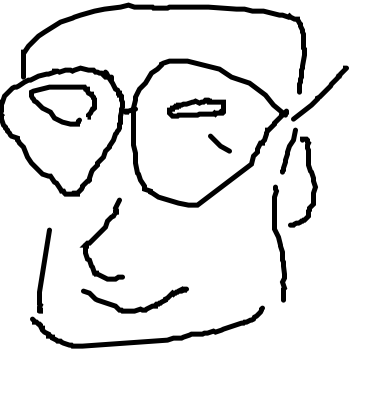
\includegraphics[width=0.2\textwidth]{art/Safari_12.png}
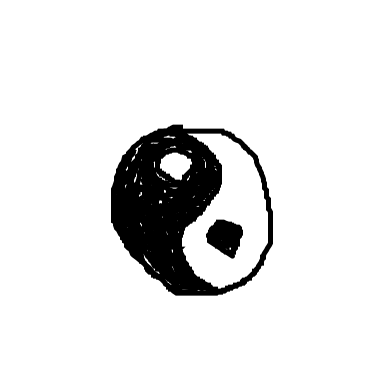
\includegraphics[width=0.2\textwidth]{art/Safari_13.png}

\includegraphics[width=0.2\textwidth]{art/Safari_14.png}

\includegraphics[width=0.2\textwidth]{art/Safari_15.png}

\includegraphics[width=0.2\textwidth]{art/Safari_16.png}
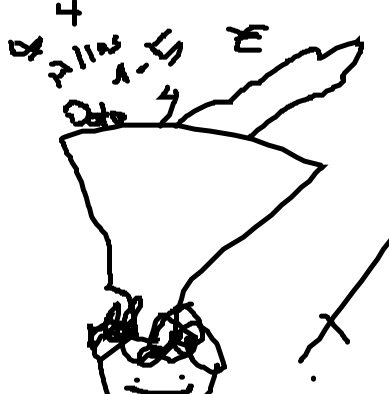
\includegraphics[width=0.2\textwidth]{art/Safari_17.png}

\includegraphics[width=0.2\textwidth]{art/Safari_18.png}

\includegraphics[width=0.2\textwidth]{art/Safari_19.png}
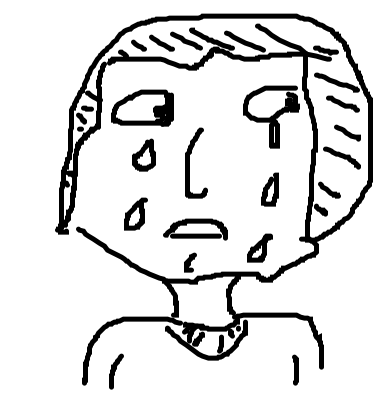
\includegraphics[width=0.2\textwidth]{art/Safari_2.png}
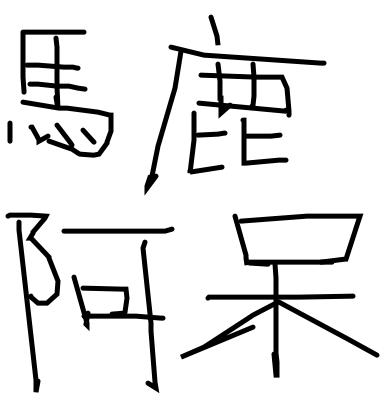
\includegraphics[width=0.2\textwidth]{art/Safari_20.png}
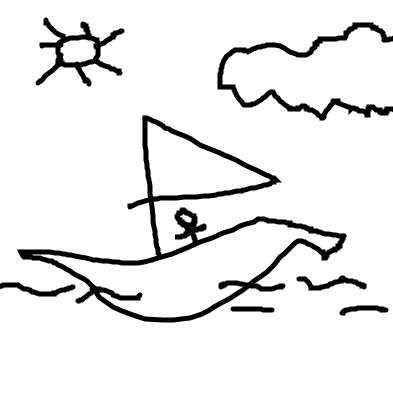
\includegraphics[width=0.2\textwidth]{art/Safari_21.png}

\includegraphics[width=0.2\textwidth]{art/Safari_22.png}
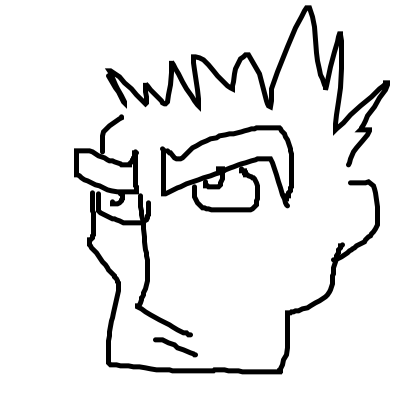
\includegraphics[width=0.2\textwidth]{art/Safari_23.png}

\includegraphics[width=0.2\textwidth]{art/Safari_24.png}

\includegraphics[width=0.2\textwidth]{art/Safari_25.png}
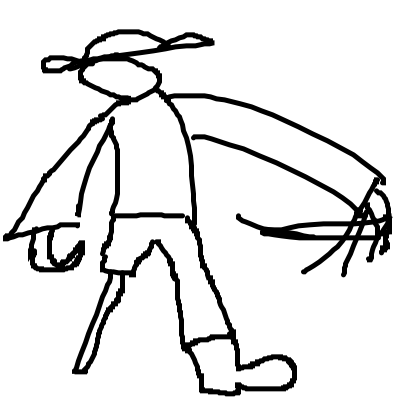
\includegraphics[width=0.2\textwidth]{art/Safari_26.png}
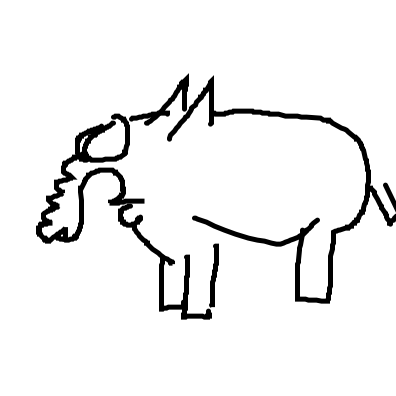
\includegraphics[width=0.2\textwidth]{art/Safari_27.png}
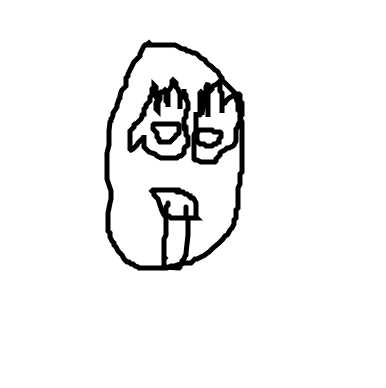
\includegraphics[width=0.2\textwidth]{art/Safari_28.png}
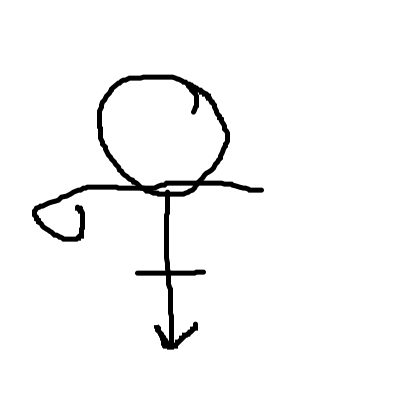
\includegraphics[width=0.2\textwidth]{art/Safari_29.png}

\includegraphics[width=0.2\textwidth]{art/Safari_3.png}

\includegraphics[width=0.2\textwidth]{art/Safari_30.png}
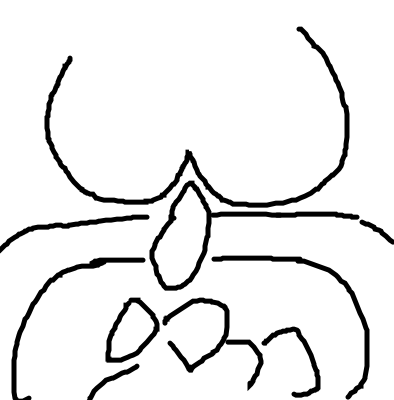
\includegraphics[width=0.2\textwidth]{art/Safari_31.png}
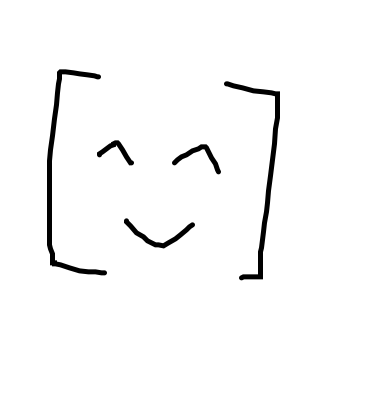
\includegraphics[width=0.2\textwidth]{art/Safari_32.png}

\includegraphics[width=0.2\textwidth]{art/Safari_33.png}
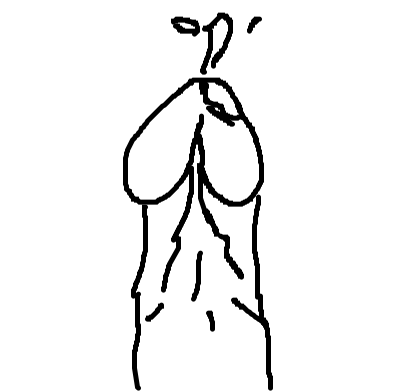
\includegraphics[width=0.2\textwidth]{art/Safari_34.png}
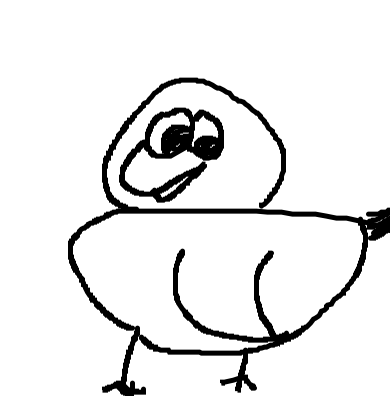
\includegraphics[width=0.2\textwidth]{art/Safari_35.png}
\includegraphics[width=0.2\textwidth]{art/Safari_36.png}
\includegraphics[width=0.2\textwidth]{art/Safari_37.png}
\includegraphics[width=0.2\textwidth]{art/Safari_38.png}
\includegraphics[width=0.2\textwidth]{art/Safari_39.png}
\includegraphics[width=0.2\textwidth]{art/Safari_4.png}
\includegraphics[width=0.2\textwidth]{art/Safari_40.png}
\includegraphics[width=0.2\textwidth]{art/Safari_41.png}
\includegraphics[width=0.2\textwidth]{art/Safari_42.png}
\includegraphics[width=0.2\textwidth]{art/Safari_43.png}
\includegraphics[width=0.2\textwidth]{art/Safari_44.png}
\includegraphics[width=0.2\textwidth]{art/Safari_45.png}
\includegraphics[width=0.2\textwidth]{art/Safari_46.png}
\includegraphics[width=0.2\textwidth]{art/Safari_47.png}
\includegraphics[width=0.2\textwidth]{art/Safari_48.png}
\includegraphics[width=0.2\textwidth]{art/Safari_49.png}
\includegraphics[width=0.2\textwidth]{art/Safari_5.png}
\includegraphics[width=0.2\textwidth]{art/Safari_50.png}
\includegraphics[width=0.2\textwidth]{art/Safari_51.png}
\includegraphics[width=0.2\textwidth]{art/Safari_52.png}
\includegraphics[width=0.2\textwidth]{art/Safari_53.png}
\includegraphics[width=0.2\textwidth]{art/Safari_54.png}
\includegraphics[width=0.2\textwidth]{art/Safari_55.png}
\includegraphics[width=0.2\textwidth]{art/Safari_56.png}
\includegraphics[width=0.2\textwidth]{art/Safari_57.png}
\includegraphics[width=0.2\textwidth]{art/Safari_58.png}
\includegraphics[width=0.2\textwidth]{art/Safari_59.png}
\includegraphics[width=0.2\textwidth]{art/Safari_6.png}
\includegraphics[width=0.2\textwidth]{art/Safari_60.png}
\includegraphics[width=0.2\textwidth]{art/Safari_61.png}
\includegraphics[width=0.2\textwidth]{art/Safari_62.png}
\includegraphics[width=0.2\textwidth]{art/Safari_63.png}
\includegraphics[width=0.2\textwidth]{art/Safari_64.png}
\includegraphics[width=0.2\textwidth]{art/Safari_65.png}
\includegraphics[width=0.2\textwidth]{art/Safari_66.png}
\includegraphics[width=0.2\textwidth]{art/Safari_67.png}
\includegraphics[width=0.2\textwidth]{art/Safari_68.png}
\includegraphics[width=0.2\textwidth]{art/Safari_69.png}
\includegraphics[width=0.2\textwidth]{art/Safari_7.png}
\includegraphics[width=0.2\textwidth]{art/Safari_70.png}
\includegraphics[width=0.2\textwidth]{art/Safari_71.png}
\includegraphics[width=0.2\textwidth]{art/Safari_72.png}
\includegraphics[width=0.2\textwidth]{art/Safari_73.png}
\includegraphics[width=0.2\textwidth]{art/Safari_74.png}
\includegraphics[width=0.2\textwidth]{art/Safari_75.png}
\includegraphics[width=0.2\textwidth]{art/Safari_76.png}
\includegraphics[width=0.2\textwidth]{art/Safari_77.png}
\includegraphics[width=0.2\textwidth]{art/Safari_78.png}
\includegraphics[width=0.2\textwidth]{art/Safari_8.png}
\includegraphics[width=0.2\textwidth]{art/Safari_9.png}


\backmatter
\chapter{Danksagungen}

% TODO
I want to thank the academy. And: Lorem ipsum dolor sit amet, consectetur adipisicing elit, sed do eiusmod tempor incididunt ut labore et dolore magna aliqua. Ut enim ad minim veniam, quis nostrud exercitation ullamco laboris nisi ut aliquip ex ea commodo consequat. Duis aute irure dolor in reprehenderit in voluptate velit esse cillum dolore eu fugiat nulla pariatur. Excepteur sint occaecat cupidatat non proident, sunt in culpa qui officia deserunt mollit anim id est laborum.

% TODO foo

%!TEX root = /Users/daniel/Documents/thesis/thesis.tex
\bibliographystyle{natdin}
\cleardoublepage
\phantomsection
\addcontentsline{toc}{chapter}{Literaturverzeichnis}
\bibliography{books,papers,web}

% \cleardoublepage
% \phantomsection
% \addcontentsline{toc}{chapter}{Abbildungsverzeichnis}
\listoffigures    % Abbildungsverzeichnis
% \cleardoublepage
% \phantomsection
% \addcontentsline{toc}{chapter}{Tabellenverzeichnis}
% \listoftables     % Tabellenverzeichnis
% \cleardoublepage
% \phantomsection
% \addcontentsline{toc}{chapter}{Algorithmenverzeichnis}
\listofalgorithms

\end{document}

